



In this chapter, I evaluate my proposed framework on Bipolar Disorder (BD) recognition. I first describe the baseline system with baseline features against which the proposed framework compares. I then present the experimental results of the Deep Denoising Autoencoders (DDAEs) on audio-visual modalities and document embeddings on text modality respectively, and the final decision is obtained with early fusion strategy, making use of all available modalities. The visualization of reconstructed visual input and embedding space is given for the qualitative analysis. I conclude the chapter with the comparison with other frameworks proposed in AVEC2018. 




\section{Baseline}

For the following experiments, I build a baseline system with Random Forest (RF) classifiers and baseline features presented in AVEC2018 \cite{ringeval2018}.

\subsection{Baseline Features}

As mentioned in Chapter \ref{ch:background} Section \ref{sec:bp-corpus}, the Turkish Audio-Visual Bipolar Disorder (BD) Corpus is recently introduced \cite{cciftcci2018}, which includes pre-partitioned training, development and test sets. The availability of the dataset is upon request while labels for the test set cannot be accessed unless participating in the AVEC2018 challenge. Besides, based on the statistics I obtained on my version of the dataset, the number of recordings in Table \ref{tab:recording_length} cannot be verified \cite{cciftcci2018} as there are only 54 samples without labels in the test partition. The imbalance between three classes is noted that there are more recordings of hypo-mania and mania than those of remission.


\begin{table}[ht]
    \centering
    \caption{Recording statistics for mania patients with different symptoms and healthy controls}
    \small
    \begin{tabular}{l|p{4cm}|p{2cm}|p{2cm}}
         \Xhline{2\arrayrulewidth}
         Diagnosis & Number of recordings in train/dev/test set & Average Time (s) & Standard Deviation \\
         \hline
         Remission & 25/18/NA & 151.9 & 65.4 \\
         \hline
         Hypo-mania & 38/21/NA & 221.1 & 171.4 \\
         \hline
         Mania & 41/21/NA & 276.4 & 246.3 \\
         \Xhline{2\arrayrulewidth}
    \end{tabular}
    \label{tab:recording_length}
\end{table}


Therefore, in the following experiments, I focus my framework on the training and development sets, whose results can be directly compared with the competing frameworks \cite{yang2018, du2018, xing2018, syed2018} in AVEC2018, and then U cross-validate our framework on all the available data for the analysis of generalization.

The baseline features used in AVEC2018 includes MFCC features, eGeMAPS features, and Bag-of-Audio-Words (BoAW) features for acoustic modality, and FAU features and Bag-of-Visual-Words (BoVW) features for visual modality. MFCC features are computed at the frame level while eGeMAPS are computed at speaker turn level that however can be aligned with other modalities given the frame time. FAU features are session-level functionals of action units over each video session, which include the mean, standard-deviation, and the relative position of the maximum. BoAW and BoVW are generated following the BoW technique, described in Chapter \ref{ch:design} Section \ref{sec:fisher}, using frame-level LLDs: MFCC features and FAU features respectively. 


\subsection{Baseline Systems}

With the baseline features available, Random Forest (RF) classifiers are fine-tuned with the following hyperparameters to obtain the optimal frame-level baseline results: the number of trees ($N$), the maximum depth of each tree ($D$) and the maximum portion of features used in each split ($S$). The objective metric used in the tuning process is the unweighted average recall (UAR). Furthermore, the training data of the minority class, remission, is replicated to be balanced with other classes \cite{ringeval2018}.

After fine-tuning and training, the frame-level results for each feature are obtained. To obtain session-level decisions, I apply a simple majority voting strategy to the baseline systems using features other than FAU, which nevertheless does not take into account the global information or temporary information of each video session.  Because of the imbalanced dataset, I measure the performance of baseline systems with recall and precision which respectively describe classifiers completeness and exactness.

\begin{table}[htb]
    \small
    \centering
    \caption{Hyperparameter settings to investigate for Random Forest classifiers}
    \begin{tabular}{l|l}
    \Xhline{2\arrayrulewidth}
        Hyperparameter & Values \\
        \hline
        Number of trees $N$ & \{100, 200, 400, 800\} \\
        Maximum depth of trees $D$ & \{2, 4, 8\} \\
        Maximum features in trees $S$ & \{0.1, 0.2, 0.4\} \\
    \Xhline{2\arrayrulewidth}
    \end{tabular}
    \label{tab:params_rf}
\end{table}


I present the experimental results of the baseline system as Table \ref{tab:baseline}. Of the metrics in Table \ref{tab:baseline}, UAR represents the unweighted average recall, which was used as the primary metric in AVEC2018, UAP represents the unweighted average precision, and F1 represents the F1 score, the harmonic mean of precision and recall: $F_1 = 2 \times \frac{precision \times recall}{precision + recall}$. The symbols F and S in the metric respectively denote frame-level and session-level. 


\begin{table}[htb]
    \small
    \centering
    \caption{Baseline systems with Random Forest classifiers on baseline features}
    \begin{tabular}{l|p{1.5cm}|p{1.9cm}|p{1.5cm}|p{1.5cm}|p{1.5cm}}
    \Xhline{2\arrayrulewidth}
    \hline
         Metric  & MFCC  & eGeMAPS & BoAW & FAU  & BoVW \\
         \hline
         UAR (F) & 0.414 & 0.396 & 0.443 & -     & 0.452 \\
         UAR (S) & 0.413 & 0.455 & \textbf{0.489} & 0.481 & 0.452 \\
         UAP     & 0.410 & 0.370 & 0.439 & \textbf{0.528} & 0.445 \\
         F1      & 0.411 & 0.408 & 0.463 & \textbf{0.503} & 0.448 \\
    \hline
    \Xhline{2\arrayrulewidth}
    \end{tabular}
    \label{tab:baseline}
\end{table}


As shown in Table \ref{tab:baseline}, BoAW-based baseline system outperforms others with an UAR at 0.489 while MFCC-based baseline the UAR is the lowest at only 0.413. It is noticeable that the baseline using FAU features has the second highest UAR score along with the highest UAP, resulting in the highest F1 score. The BoAW-based and FAU-based systems are selected as the baseline for the following experiments.





\section{Audio-Visual Modalities}

To validate the feature learning of audio-visual modalities, the proposed Deep Denoising Autoencoders (DDAEs) are evaluated with the performance in the supervised learning task, BD classification. As the number of Gaussians (16 or 32) in Fisher Vectors (FVs) is investigated, there would be 36 hyperparameter settings for just the Unimodal DDAE architectures. Thus I focus on the hyperparameters of DDAEs, whose results are based on the better-performing Fisher Vector, using either 16 or 32 kernels in the Gaussian Mixture Models. Furthermore, to solely evaluate the latent representations of DDAEs and the FVs, the classification performance is measured with the same fine-tuned Random Forest (RF) classifiers as the baseline system. The complete experimental results are attached in Appendix \ref{sec:DDAE_full}. As Chapter \ref{ch:design} Section \ref{sec:DDAE}, the Unimodal DDAEs (uni-DDAEs), Bimodal DDAEs (bi-DDAEs), and Multimodal DDAEs (multi-DDAEs) are individually evaluated in the following subsections.

\subsection{Assessment of Unimodal Feature Learning}

I first present the experimental results for unimodal feature learning in Table \ref{tab:unimodal_res}, in which DDAEs are trained on unimodal data: facial landmarks, MFCC features or eGeMAPS features. A Monte Carlo permutation test is additionally implemented for the following experiments to evaluate the probability that the difference between baseline systems and proposed systems occurs by random chance. As there are 60 samples in the development set, the number of random permutations is pre-fixed to 5000 instead of $2^{60}$.


\begin{table}[htb]
    \small
    \centering
    \caption{Comparison of proposed Unimodal DDAE architectures (selected experimental results). The best performance is in \textbf{bold} for each metric and the baseline results are attached.}
    \begin{tabular}{l|l|p{1.25cm}|l|p{1.2cm}|l|l|l}
    \Xhline{2\arrayrulewidth}
        Index & Acoustic feature & Hidden ratio & Noise & GMM kernel & UAR & UAP & F1 \\
        \hline
        (1)  & Landmarks & 0.4 & 0.1 & 16 & 0.582 & 0.590 & 0.586 \\
        (2)  & Landmarks & 0.4 & 0.2 & 32 & \textbf{0.624} & \textbf{0.692} & \textbf{0.656} \\
        (3)  & Landmarks & 0.4 & 0.4 & 32 & 0.614 & 0.622 & 0.618 \\
        (4)  & Landmarks & 0.5 & 0.1 & 16 & 0.585 & 0.628 & 0.606 \\
        (5)  & Landmarks & 0.5 & 0.2 & 32 & 0.606 & 0.635 & 0.620 \\
        (6)  & Landmarks & 0.5 & 0.4 & 32 & 0.611 & 0.620 & 0.615 \\
        \hline
        (7)  & MFCC & 0.4 & 0.1 & 32 & \textbf{0.587} & \textbf{0.611} & \textbf{0.599} \\
        (8)  & MFCC & 0.4 & 0.2 & 32 & 0.542 & 0.562 & 0.552 \\
        (9)  & MFCC & 0.4 & 0.4 & 16 & 0.521 & 0.562 & 0.541 \\
        (10) & MFCC & 0.5 & 0.1 & 16 & 0.550 & 0.575 & 0.562 \\
        (11) & MFCC & 0.5 & 0.2 & 32 & 0.561 & 0.607 & 0.583 \\
        (12) & MFCC & 0.5 & 0.4 & 16 & 0.545 & 0.585 & 0.564 \\
        \hline
        (13) & eGeMAPS & 0.4 & 0.1 & 16 & 0.561 & 0.591 & 0.576 \\
        (14) & eGeMAPS & 0.4 & 0.2 & 32 & 0.524 & 0.532 & 0.528 \\
        (15) & eGeMAPS & 0.4 & 0.4 & 32 & 0.511 & 0.563 & 0.536 \\
        (16) & eGeMAPS & 0.5 & 0.1 & 32 & \textbf{0.632} & \textbf{0.654} & \textbf{0.637} \\
        (17) & eGeMAPS & 0.5 & 0.2 & 32 & 0.590 & 0.619 & 0.604 \\
        (18) & eGeMAPS & 0.5 & 0.4 & 32 & 0.563 & 0.585 & 0.574 \\
        \hline
        & \multicolumn{4}{l|}{Baseline (BoAW)} & 0.489 & 0.439 & 0.463 \\
        & \multicolumn{4}{l|}{Baseline (FAU)} & 0.481 & 0.528 & 0.503 \\
    \Xhline{2\arrayrulewidth}
    \end{tabular}
    \label{tab:unimodal_res}
\end{table}


In Table \ref{tab:unimodal_res}, the results show an improvement from the baseline system. Specifically, for facial landmarks, the best-performing uni-DDAE reaches up to 0.624 UAR with 0.658 F1 score ((2) in Table \ref{tab:unimodal_res}) and for eGeMAPS features, the uni-DDAEs obtain a higher UAR at 0.632 with 0.637 F1 score ((16) in Table \ref{tab:unimodal_res}). On the other hand, UAR for uni-DDAEs using MFCC features is lower than other uni-DDAEs at only 0.587 but higher than the best-performing baseline as (7) seen in Table \ref{tab:unimodal_res}. With respect to uni-DDAEs and baseline systems using same features, (7) performs significantly between than the baseline using MFCC ($p = 0.0002 < 0.001$) but (16) does not outperform the baseline using eGeMAPS significantly ($p = 0.4459 > 0.1$).

It is clear that a compact size benefits latent representations for facial landmarks because the DDAEs with hidden ratio 0.4 (21-dimensional representations) show better performance than those with hidden ratio 0.5 (34-dimensional representations). While the smaller hidden ratio for DDAEs using eGeMAPS features affects the performance negatively, the hidden ratio seems to have little impact on the performance of DDAEs using MFCC features. 

The noise appended to the input forces the autoencoders to learn more robust features \cite{vincent2008}, which can be validated in DDAEs with facial landmarks as 0.2 noise leads to a higher F1 score than 0.1 noise. Nevertheless, to the acoustic features, more noise causes F1 score to decrease.

To the acoustic features, eGeMAPS features demonstrate a better performance over MFCC features in uni-DDAEs. The best-performing RF classifiers ((7) and (16) in Table \ref{tab:unimodal_res}) show a performance gap of 0.045 in UAR and 0.038 in F1 score but they fail to significantly differ from each other with $p = 0.16 > 0.1$


\begin{figure}
    \centering
    \small
    \begin{minipage}[c]{0.31\linewidth}
    \centering
    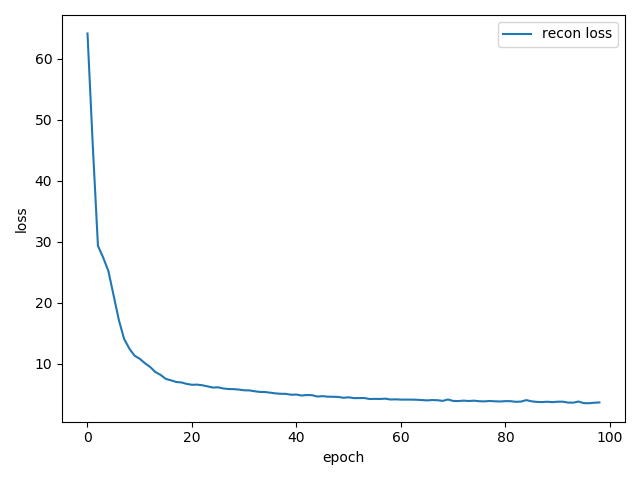
\includegraphics[width=\textwidth]{images/results/unimodal_landmark_hidden040_batch1024_epoch100_noise02.png} \\
    Facial Landmarks
    \end{minipage}
    \begin{minipage}[c]{0.31\linewidth}
    \centering
    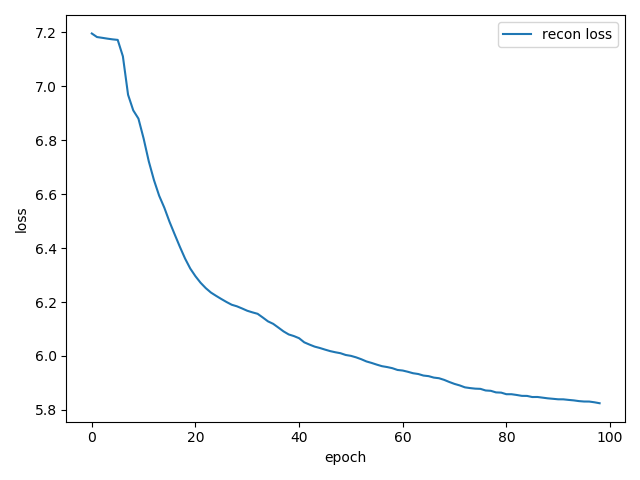
\includegraphics[width=\textwidth]{images/results/unimodal_mfcc_hidden040_batch1024_epoch100_noise01.png} \\
    MFCC
    \end{minipage}
    \begin{minipage}[c]{0.31\linewidth}
    \centering
    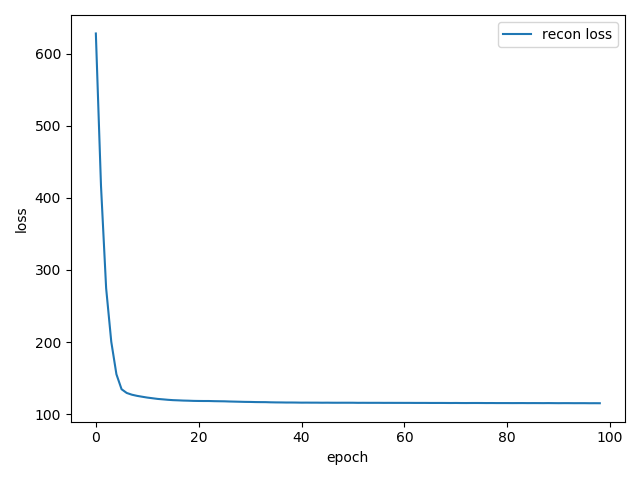
\includegraphics[width=\textwidth]{images/results/unimodal_egemaps_hidden050_batch1024_epoch100_noise01.png} \\
    eGeMAPS
    \end{minipage}
    \caption{Loss during training for Unimodal DDAE}
    \label{fig:loss_unimodal}
\end{figure}

The reconstruction loss during the training processing is visualized for the best-performing uni-DDAEs ((2), (7) and (16) in Table \ref{tab:unimodal_res}) using different features as Figure \ref{fig:loss_unimodal}. As discussed in Chapter \ref{ch:design} Section \ref{sec:DDAE}, the loss function is set the mean squared error (MSE) instead of binary cross-entropy (BCE) as I find that with BCE, the loss cannot be minimized in the training and the latent representations prove meaningless in the classification. Although three uni-DDAEs succeed to minimize the reconstruction loss, it is worthy to notice the different ranges of loss values, which is discussed in the bimodal feature learning.

The full version of experimental results for uni-DDAEs refers to \ref{tab:unimodal_res_full}.




\subsection{Assessment of Bimodal Feature Learning}

In the bimodal feature learning, the visual modality is fixed to facial landmarks and the acoustic modality is investigated on either MFCC features or eGeMAPS features. As seen in Table \ref{tab:bimodal_res}, bi-DDAEs with MFCC as acoustic feature generally have better performance than those with eGeMAPS. When compared to the best-performing uni-DDAEs with facial landmarks and MFCC, a performance gain is observed in bi-DDAEs with MFCC that the joint representations across two modalities demonstrate more discriminative for BD recognition. However, bi-DDAEs with eGeMAPS show a performance drop instead that the F1 score is lower than either uni-DDAE using acoustic or visual modality. This finding may explained with the loss during training for uni-DDAEs (Figure \ref{fig:loss_unimodal}) and bi-DDAEs (Figure \ref{fig:loss_bimodal}). As displayed in Figure \ref{fig:loss_unimodal}, the loss for facial landmarks decreases to approximately 5.0, within the same scale of MFCC features, while the loss for eGeMAPS features starts at more than 600.0 and is finally minimized at 115.0, which is much larger than the scale for other two features. Therefore, in the bi-DDAEs with eGeMAPS, the acoustic loss still starts at a high value and causes the joint loss higher than the visual loss. More specifically, the acoustic loss is reduced to around 83.4 while the visual loss to around 27.0. On the other hand, the acoustic and visual loss in bi-DDAEs using MFCC decline with the same pattern and end at approximately 10.3 and 6.3 respectively.

\begin{figure}
    \centering
    \small
    \begin{minipage}[c]{0.48\linewidth}
    \centering
    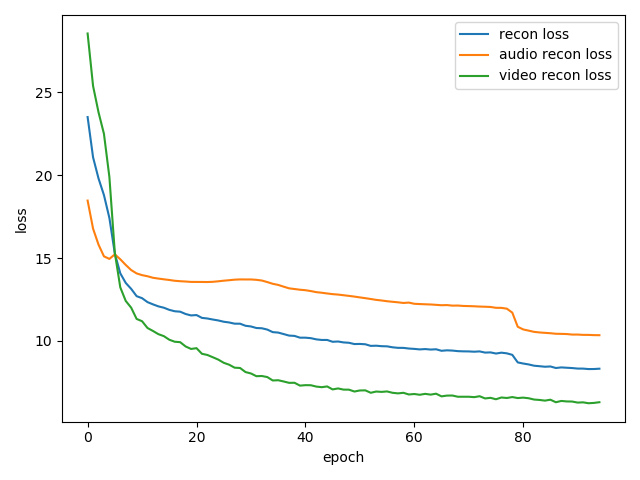
\includegraphics[width=\textwidth]{images/results/bimodal_aligned_mfcc_hidden040_batch1024_epoch100_noise01.png} \\
    MFCC
    \end{minipage}
    \begin{minipage}[c]{0.48\linewidth}
    \centering
    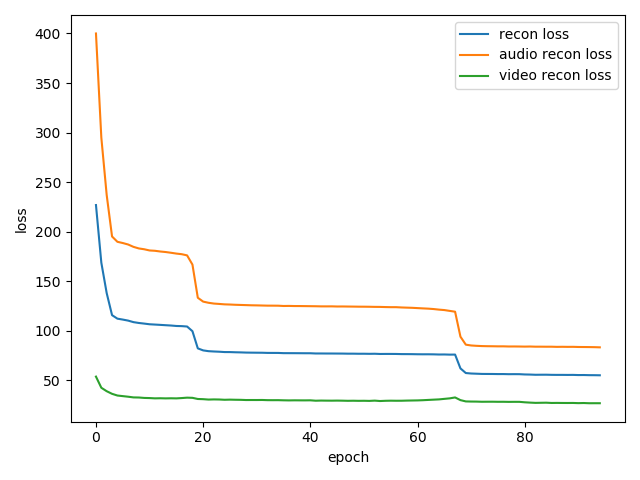
\includegraphics[width=\textwidth]{images/results/bimodal_aligned_egemaps_hidden050_batch1024_epoch100_noise01.png} \\
    eGeMAPS
    \end{minipage}
    \caption{Loss during training for Bimodal DDAE}
    \label{fig:loss_bimodal}
\end{figure}

In addition to the better performance of bi-DDAEs, the kernels of GMMs has proven a considerable impact on the classification, which in bi-DDAEs are mostly 32. Nonetheless, the bi-DDAE (1) in Table \ref{tab:bimodal_res} with 16 GMM kernels has an UAR at 0.492 and F1 score at 0.473, much lower than the same setting with 32 GMM kernels (Table \ref{tab:bimodal_res_full}). 

The size of latent representations affects the performance the same way as the uni-DDAEs on MFCC and eGeMAPS that bi-DDAEs on MFCC favour a smaller hidden ratio while those on eGeMAPS favour a larger hidden ratio. In terms of noise, much noise (more than 0.1) is observed to hurt the performance. It is worth pointing out that bi-DDAE (1) in Table \ref{tab:bimodal_res} slightly outperforms the framework proposed by \cite{syed2018} in AVEC2018.

The full version of experimental results for Bimodal DDAEs refers to \ref{tab:bimodal_res_full}.

\begin{table}[htb]
    \small
    \centering
    \caption{Comparison of proposed Bimodal DDAE architectures (selected experimental results). The best performance is in \textbf{bold} for each metric, and the baseline results and best-performing results for Unimodal DDAEs are attached.}
    \begin{tabular}{l|p{1.8cm}|p{1.25cm}|l|p{1.2cm}|l|l|l}
    \Xhline{2\arrayrulewidth}
        Index & Acoustic feature & Hidden ratio & Noise & GMM kernel & UAR & UAP & F1 \\
        \hline
        (1)  & MFCC  & 0.4 & 0.1 & 32 & \textbf{0.656} & \textbf{0.677} & \textbf{0.666} \\
        (2)  & MFCC  & 0.4 & 0.2 & 16 & 0.632 & 0.644 & 0.638 \\
        (3)  & MFCC  & 0.4 & 0.4 & 32 & 0.447 & 0.462 & 0.454 \\
        (4)  & MFCC  & 0.5 & 0.1 & 32 & 0.505 & 0.524 & 0.514 \\
        (5)  & MFCC  & 0.5 & 0.2 & 32 & 0.489 & 0.586 & 0.533 \\
        (6)  & MFCC  & 0.5 & 0.4 & 32 & 0.545 & 0.561 & 0.553 \\
        \hline
        (7)  & eGeMAPS & 0.4 & 0.1 & 32 & 0.566 & 0.569 & 0.567 \\
        (8)  & eGeMAPS & 0.4 & 0.2 & 32 & 0.516 & 0.600 & 0.555 \\
        (9)  & eGeMAPS & 0.4 & 0.4 & 32 & 0.511 & 0.538 & 0.524 \\
        (10) & eGeMAPS & 0.5 & 0.1 & 16 & \textbf{0.566} & \textbf{0.611} & \textbf{0.587} \\
        (11) & eGeMAPS & 0.5 & 0.2 & 16 & 0.479 & 0.497 & 0.488 \\
        (12) & eGeMAPS & 0.5 & 0.4 & 32 & 0.519 & 0.607 & 0.560 \\
        \hline
        & \multicolumn{4}{l|}{Baseline (BoAW)} & 0.489 & 0.439 & 0.463 \\
        & \multicolumn{4}{l|}{Baseline (FAU)} & 0.481 & 0.528 & 0.503 \\
        \hline
        & \multicolumn{4}{l|}{Best Unimodal DDAE (Landmarks)} & 0.624 & 0.692 & 0.656 \\
        & \multicolumn{4}{l|}{Best Unimodal DDAE (MFCC)} & 0.587 & 0.611 & 0.599 \\
        & \multicolumn{4}{l|}{Best Unimodal DDAE (eGeMAPS)} & 0.632 & 0.654 & 0.637 \\
    \Xhline{2\arrayrulewidth}
    \end{tabular}
    \label{tab:bimodal_res}
\end{table}



\subsection{Assessment of Multimodal Feature Learning}

For multimodal feature learning, a total of five modalities are input into the multi-DDAEs including acoustic features (either MFCC or eGeMAPS), facial landmarks, eye gaze, head pose, and action units. As shown in Table \ref{tab:multimodal_res}, multi-DDAE (1) using MFCC features performs the best, with 0.656 UAR and 0.667 F1 score, but it fails to outperform the best-performing bi-DDAE on the same features because UAR are 0.656 for both models and $p = 0.69 >> 0.1$ in the permutation test. However, a small increase is obtained in other multi-DDAEs using MFCC features when compared with bi-DDAEs with the same hyperparameter setting. This demonstrates the \textit{complementarity} of multi-modal data that modality-specific information has been appended to the system by addition modality: eye gaze, head pose, and action units. Nonetheless, it is also noticeable that only multi-DDAE (2) in Table \ref{tab:multimodal_res} shows a decrease in all metrics compared with bi-DDAE (2) in Table \ref{tab:bimodal_res}. 

For eGeMAPS features, there is a considerable gain in UAR of multi-DDAEs when compared with bi-DDAEs. The best-performing bi-DDAE with eGeMAPS has an UAR of 0.566 while multi-DDAE (10) in Table \ref{tab:multimodal_res} reaches an UAR of 0.622 (0.056 higher). and it performs significantly better than the former with $p = 0.05$ in the permutation test.

The multi-DDAEs follow the same pattern as bi-DDAEs in the hyperparameter, hidden ratio, that multi-DDAEs using MFCC tend to perform better with a more compact size of the latent representation. The same pattern is found in another hyperparameter, noise, that much noise negatively affects the performance, such as a dramatic drop of 0.08 in F1 score when compared (8) with (9).

\begin{figure}
    \centering
    \small
    \begin{minipage}[c]{0.48\linewidth}
    \centering
    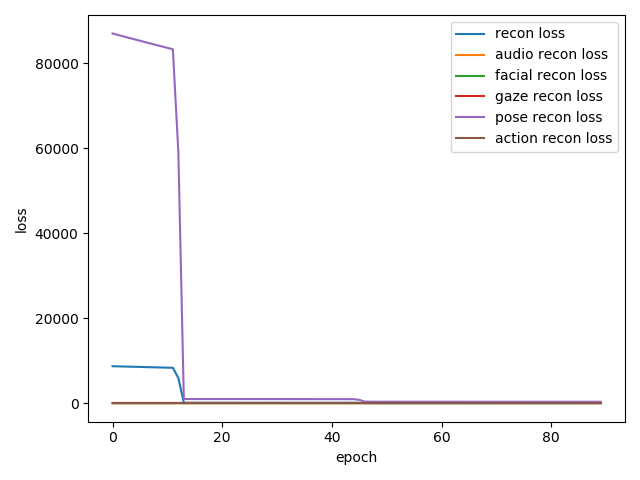
\includegraphics[width=\textwidth]{images/results/multimodal_aligned_mfcc_hidden040_batch1024_epoch100_noise01_full.png}
    \end{minipage}
    \begin{minipage}[c]{0.48\linewidth}
    \centering
    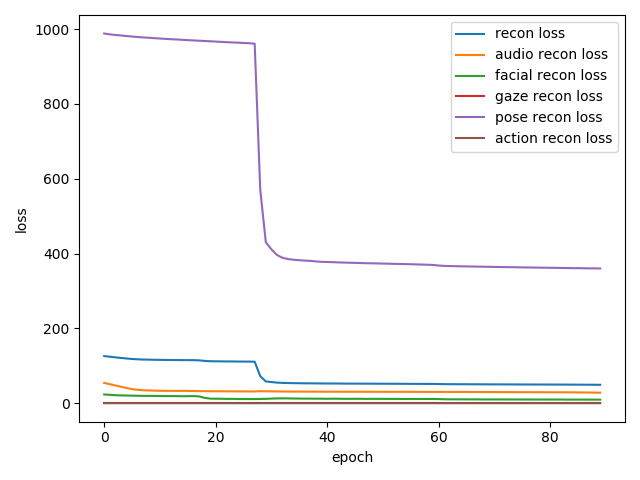
\includegraphics[width=\textwidth]{images/results/multimodal_aligned_egemaps_hidden050_batch1024_epoch100_noise01_full.png}
    \end{minipage}
    \begin{minipage}[c]{0.48\linewidth}
    \centering
    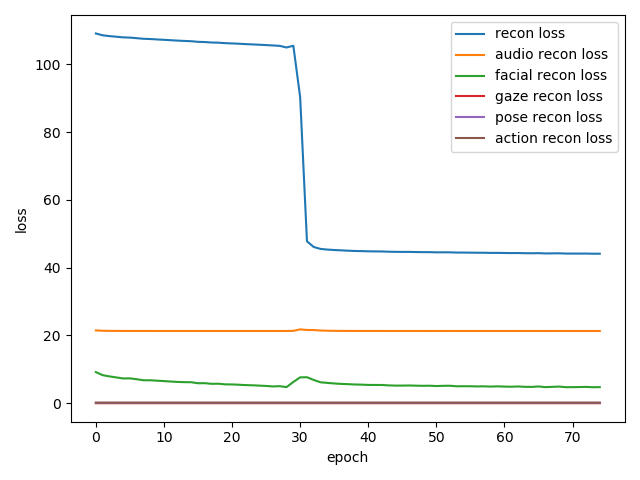
\includegraphics[width=\textwidth]{images/results/multimodal_aligned_mfcc_hidden040_batch1024_epoch100_noise01.png} \\
    MFCC
    \end{minipage}
    \begin{minipage}[c]{0.48\linewidth}
    \centering
    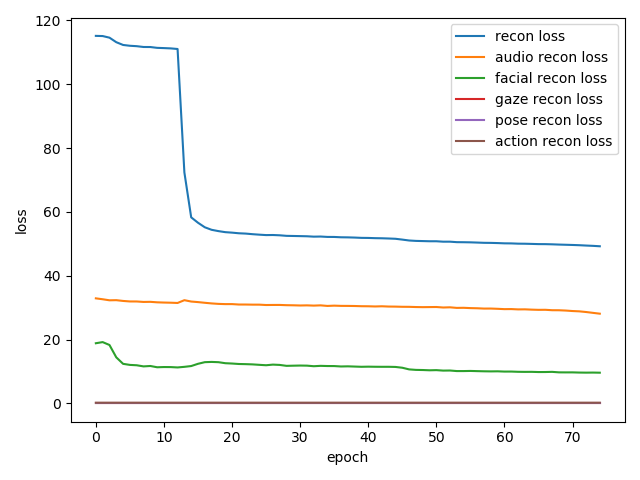
\includegraphics[width=\textwidth]{images/results/multimodal_aligned_egemaps_hidden050_batch1024_epoch100_noise01.png} \\
    eGeMAPS
    \end{minipage}
    \caption{Loss during training for Multimodal DDAE (The reconstruction loss for modality head pose is removed in the second-row graphs)}
    \label{fig:loss_multimodal}
\end{figure}

With the visualization of reconstruction loss in multi-DDAEs (1) and (10) in Table \ref{tab:multimodal_res}, some findings can help to explain little improvement of multi-DDAEs using MFCC. In Figure \ref{fig:loss_multimodal}, the two images on the upper row show the reconstruction loss of all five modalities during training and the two images on the lower row focus on the modalities except head pose, which is preset to zero. Head pose is demonstrated difficult to be reconstructed via the multi-DDAEs as the head pose loss is relatively larger than other modalities. 

The full version of experimental results for Multimodal DDAEs refers to \ref{tab:multimodal_res_full}.



\begin{table}[htb]
    \small
    \centering
    \caption{Comparison of proposed Multimodal DDAE architectures (selected experimental results). The best performance is in \textbf{bold} for each metric, and the baseline results and best-performing results for previous DDAEs are attached.}
    \begin{tabular}{l|p{1.8cm}|p{1.25cm}|l|p{1.2cm}|l|l|l}
    \Xhline{2\arrayrulewidth}
        Index & Acoustic feature & Hidden ratio & Noise & GMM kernel & UAR & UAP & F1 \\
        \hline
        (1)  & MFCC  & 0.4 & 0.1 & 32 & \textbf{0.656} & \textbf{0.678} & \textbf{0.667} \\
        (2)  & MFCC  & 0.4 & 0.2 & 32 & 0.566 & 0.573 & 0.569 \\
        (3)  & MFCC  & 0.4 & 0.4 & 16 & 0.569 & 0.593 & 0.581 \\
        (4)  & MFCC  & 0.5 & 0.1 & 16 & 0.597 & 0.596 & 0.596 \\
        (5)  & MFCC  & 0.5 & 0.2 & 32 & 0.569 & 0.578 & 0.573 \\
        (6)  & MFCC  & 0.5 & 0.4 & 16 & 0.569 & 0.697 & 0.627 \\
        \hline
        (7)  & eGeMAPS & 0.4 & 0.1 & 16 & 0.603 & 0.717 & 0.655 \\
        (8)  & eGeMAPS & 0.4 & 0.2 & 32 & 0.585 & 0.590 & 0.587 \\
        (9)  & eGeMAPS & 0.4 & 0.4 & 16 & 0.489 & 0.514 & 0.501 \\
        (10) & eGeMAPS & 0.5 & 0.1 & 32 & \textbf{0.622} & \textbf{0.665} & \textbf{0.642} \\
        (11) & eGeMAPS & 0.5 & 0.2 & 16 & 0.574 & 0.570 & 0.572 \\
        (12) & eGeMAPS & 0.5 & 0.4 & 16 & 0.484 & 0.536 & 0.507 \\
        \hline
        & \multicolumn{4}{l|}{Baseline (BoAW)} & 0.489 & 0.439 & 0.463 \\
        & \multicolumn{4}{l|}{Baseline (FAU)} & 0.481 & 0.528 & 0.503 \\
        \hline
        & \multicolumn{4}{l|}{Best Unimodal DDAE (Landmarks)} & 0.624 & 0.692 & 0.656 \\
        & \multicolumn{4}{l|}{Best Unimodal DDAE (MFCC)} & 0.587 & 0.611 & 0.599 \\
        & \multicolumn{4}{l|}{Best Unimodal DDAE (eGeMAPS)} & 0.632 & 0.654 & 0.637 \\
        \hline
        & \multicolumn{4}{l|}{Best Bimodal DDAE (MFCC)} & 0.656 & 0.677 & 0.666 \\
        & \multicolumn{4}{l|}{Best Bimodal DDAE (eGeMAPS)} & 0.566 & 0.611 & 0.587 \\
    \Xhline{2\arrayrulewidth}
    \end{tabular}
    \label{tab:multimodal_res}
\end{table}


\subsection{Visualization}

To evaluate the denoising effect of bi-DDAEs and multi-DDAEs, the facial landmarks are selected in the visualization of the reconstructed input. Figure \ref{fig:reconstruction_biDDAE} displays the reconstruction in bi-DDAEs at two specific frames and the images of the interviewee are reserved for better illustration. It is clear that the bi-DDAE on eGeMAPS ((10) in Table \ref{tab:bimodal_res}) performs better at the denoising that the reconstructed facial landmarks are perceived closer to the original input. The bi-DDAE on MFCC ((1) in Table \ref{tab:bimodal_res}), on the other hand, does not reconstruct the facial landmarks properly but the spatial distribution is restored via the decoder part.

\begin{figure}[htb]
    \centering
    \small
    \begin{minipage}[c]{0.42\linewidth}
    \centering
    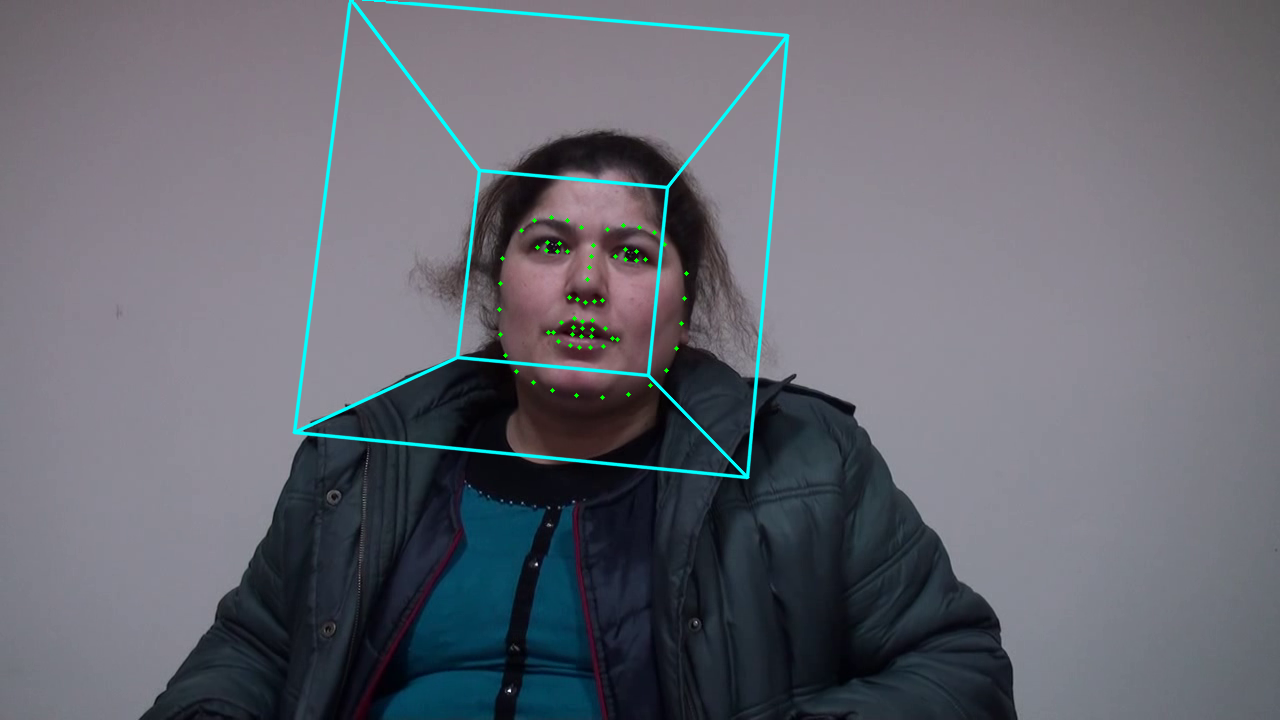
\includegraphics[width=\textwidth]{images/facial/frame_45_face_0.png} \\
    (a) original input at frame 45 (without noise)
    \end{minipage}
    \begin{minipage}[c]{0.42\linewidth}
    \centering
    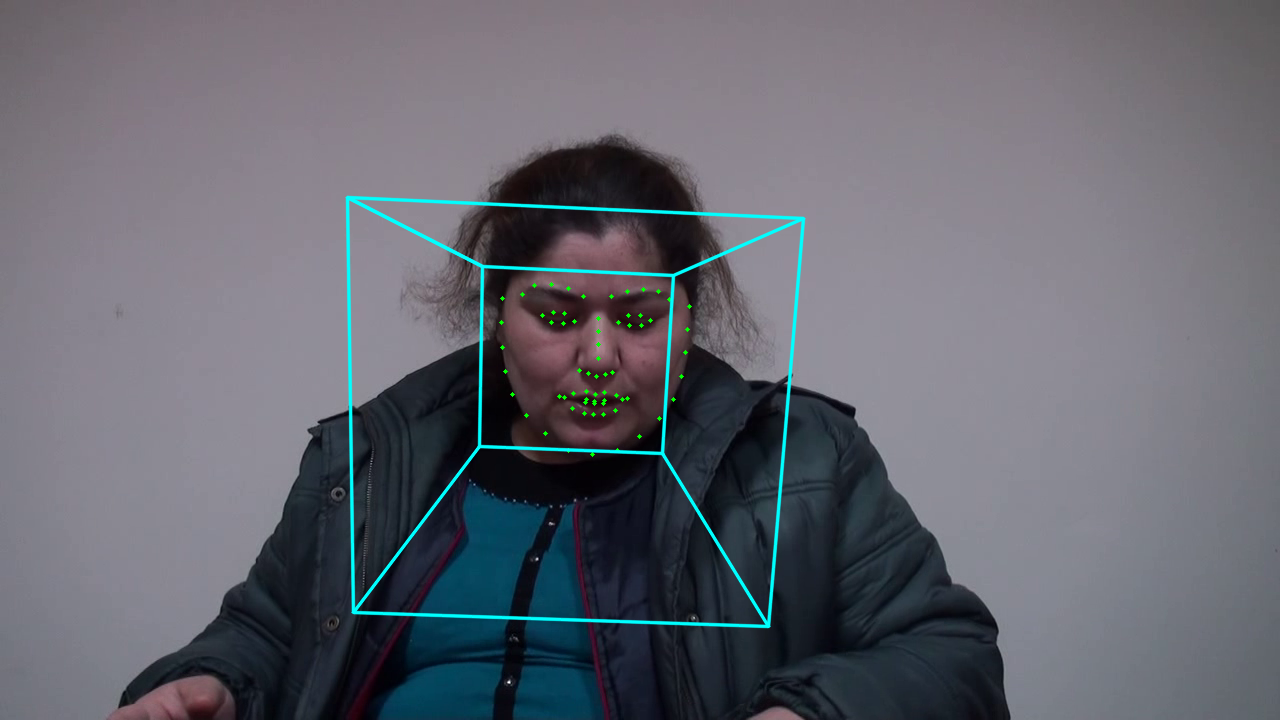
\includegraphics[width=\textwidth]{images/facial/frame_285_face_0.png} \\
    (b) original input at frame 285 (without noise)
    \end{minipage}
    \\
    \begin{minipage}[c]{0.42\linewidth}
    \centering
    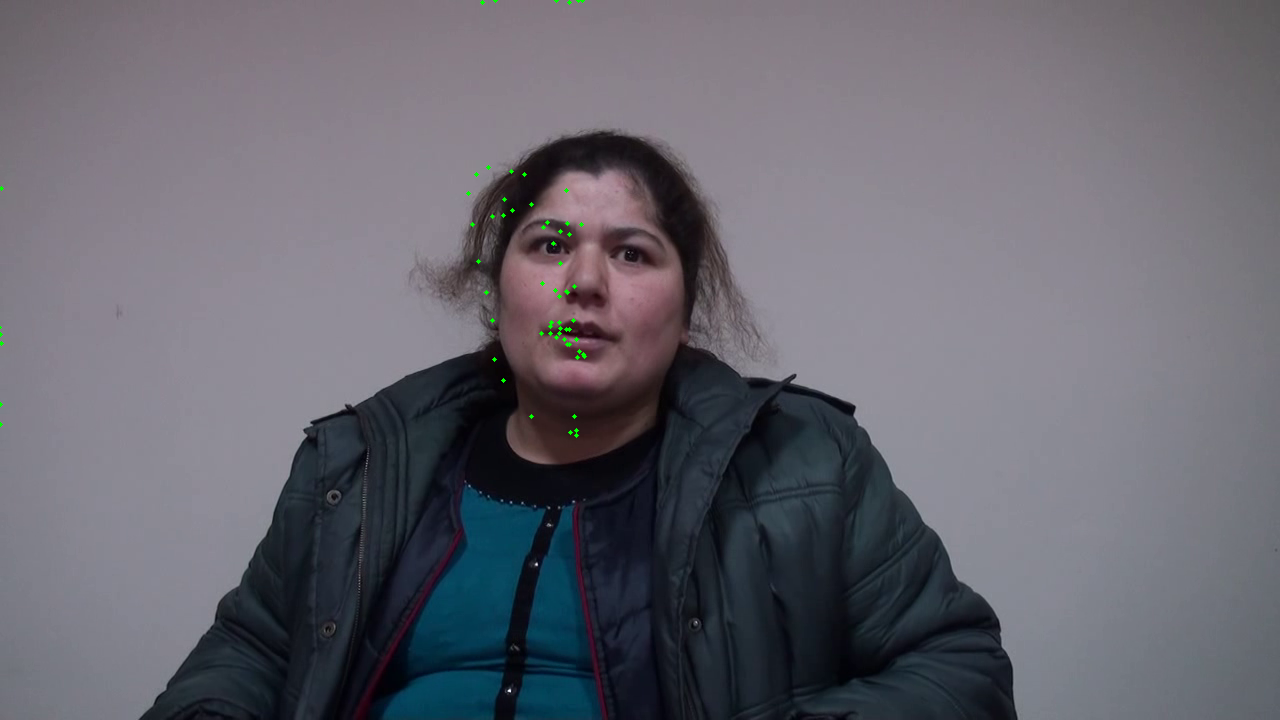
\includegraphics[width=\textwidth]{images/facial/recons_45_face_0_biDDAE_mfcc.png} \\
    (c) reconstructed input at frame 45 from (1) in Table \ref{tab:bimodal_res}
    \end{minipage}
    \begin{minipage}[c]{0.42\linewidth}
    \centering
    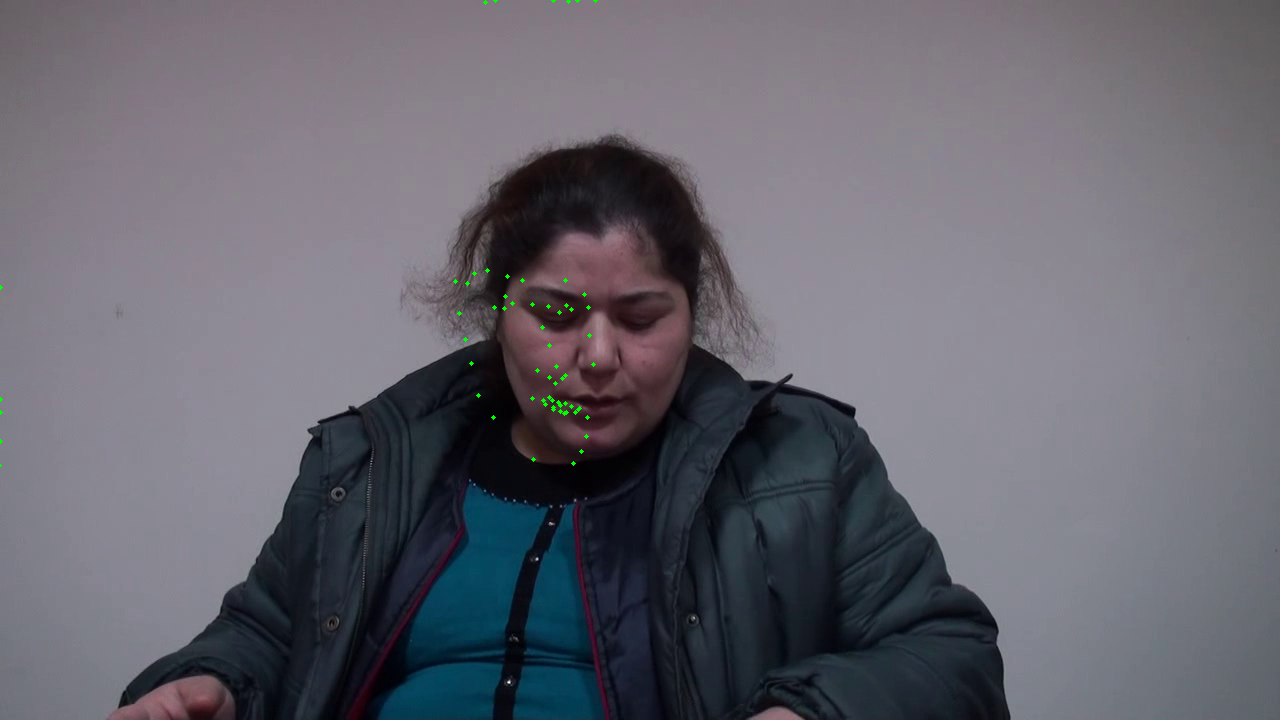
\includegraphics[width=\textwidth]{images/facial/recons_285_face_0_biDDAE_mfcc.png} \\
    (d) reconstructed input at frame 285 from (1) in Table \ref{tab:bimodal_res}
    \end{minipage}
    \\
    \begin{minipage}[c]{0.42\linewidth}
    \centering
    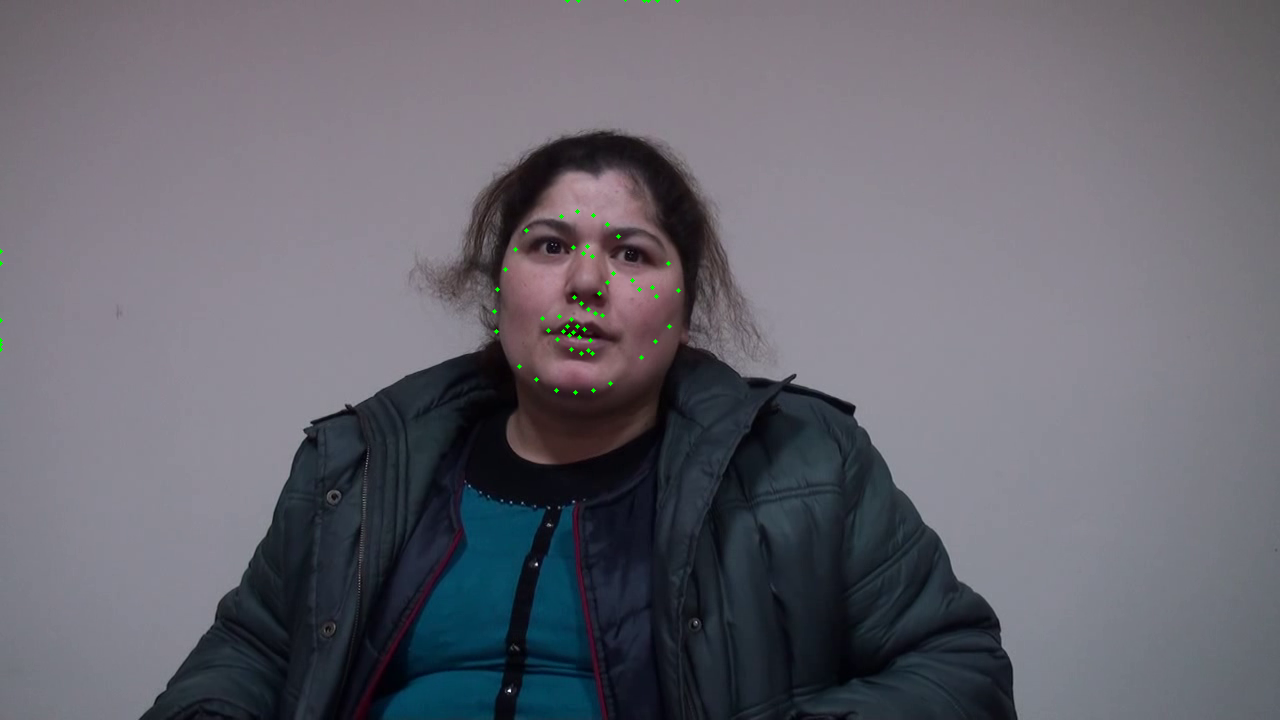
\includegraphics[width=\textwidth]{images/facial/recons_45_face_0_biDDAE_egemaps.png} \\
    (e) reconstructed input at frame 45 from (10) in Table \ref{tab:bimodal_res}
    \end{minipage}
    \begin{minipage}[c]{0.42\linewidth}
    \centering
    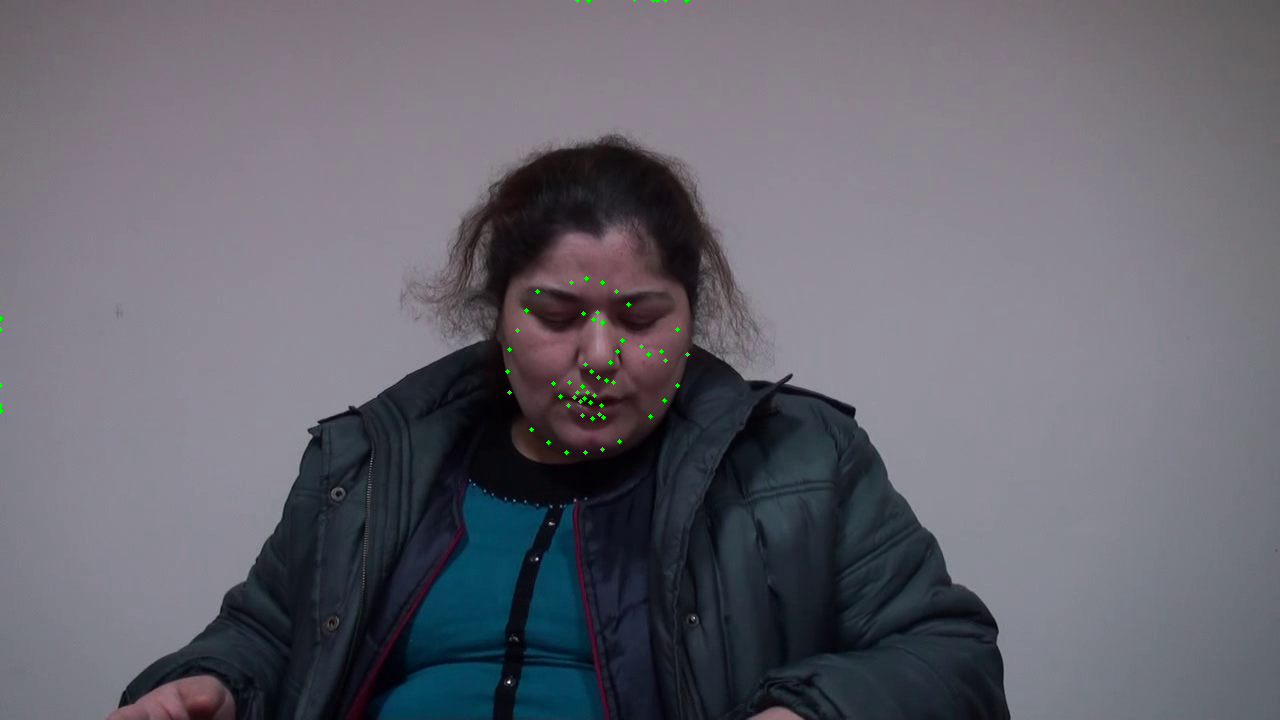
\includegraphics[width=\textwidth]{images/facial/recons_285_face_0_biDDAE_egemaps.png} \\
    (f) reconstructed input at frame 285 from (10) in Table \ref{tab:bimodal_res}
    \end{minipage}
    \caption{Reconstruction of facial landmarks in Bimodal DDAEs from noisy input}
    \label{fig:reconstruction_biDDAE}
\end{figure}

Because the head pose is relatively difficult to reconstruct as seen from Figure \ref{fig:loss_multimodal}, the reconstructed facial landmarks and head pose are visualized for multi-DDAEs in Figure \ref{fig:reconstruction_multiDDAE}. (c) and (d) in Figure \ref{fig:reconstruction_multiDDAE} demonstrates that the reconstruction of these two modalities is not intuitively convincing and the involvement of more modalities makes it more difficult to reconstruct one single modality. Moreover, the head pose in (a) and (b) is different from each other while the reconstructions (c) and (d) approximately show no difference. Similar conclusions could be drawn to multi-DDAEs on eGeMAPS ((10) in Table \ref{tab:multimodal_res}). 

\begin{figure}[htb]
    \centering
    \small
    \begin{minipage}[c]{0.42\linewidth}
    \centering
    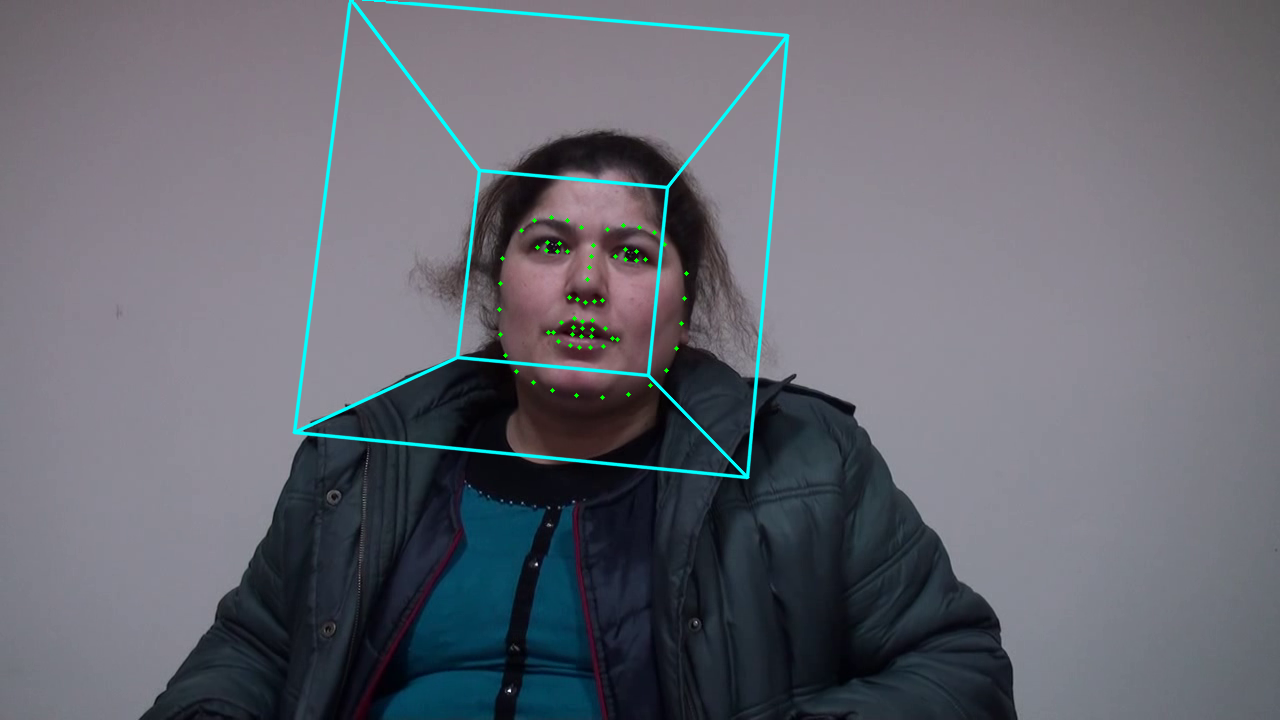
\includegraphics[width=\textwidth]{images/facial/frame_45_face_0.png} \\
    (a) original input at frame 45 (without noise)
    \end{minipage}
    \begin{minipage}[c]{0.42\linewidth}
    \centering
    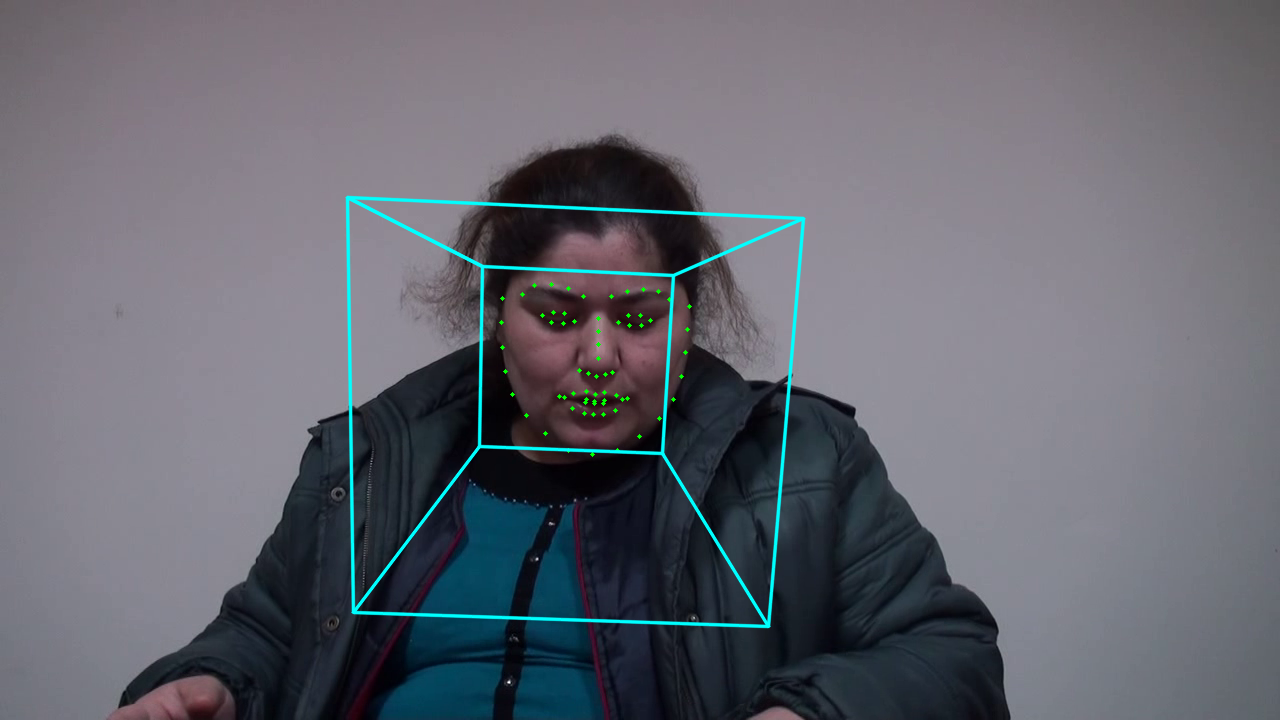
\includegraphics[width=\textwidth]{images/facial/frame_285_face_0.png} \\
    (b) original input at frame 285 (without noise)
    \end{minipage}
    \\
    \begin{minipage}[c]{0.42\linewidth}
    \centering
    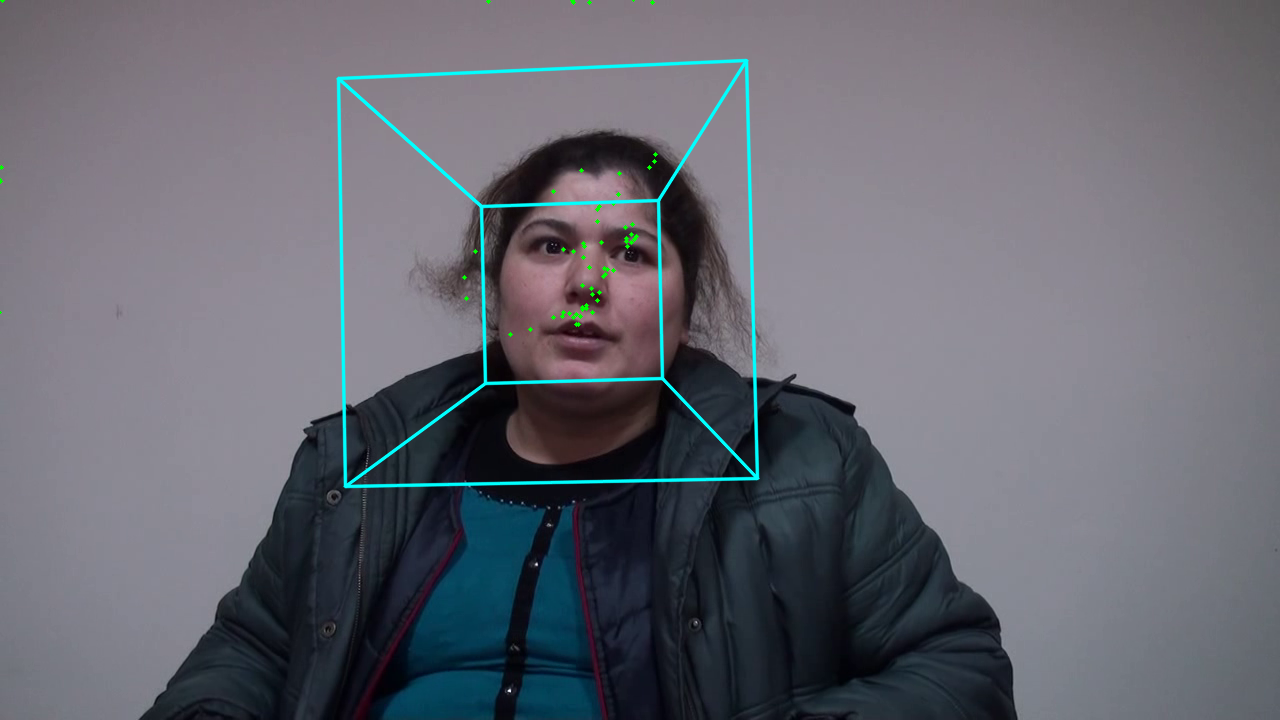
\includegraphics[width=\textwidth]{images/facial/recons_45_face_0_multiDDAE_mfcc.png} \\
    (c) reconstructed input at frame 45 from (1) in Table \ref{tab:multimodal_res}
    \end{minipage}
    \begin{minipage}[c]{0.42\linewidth}
    \centering
    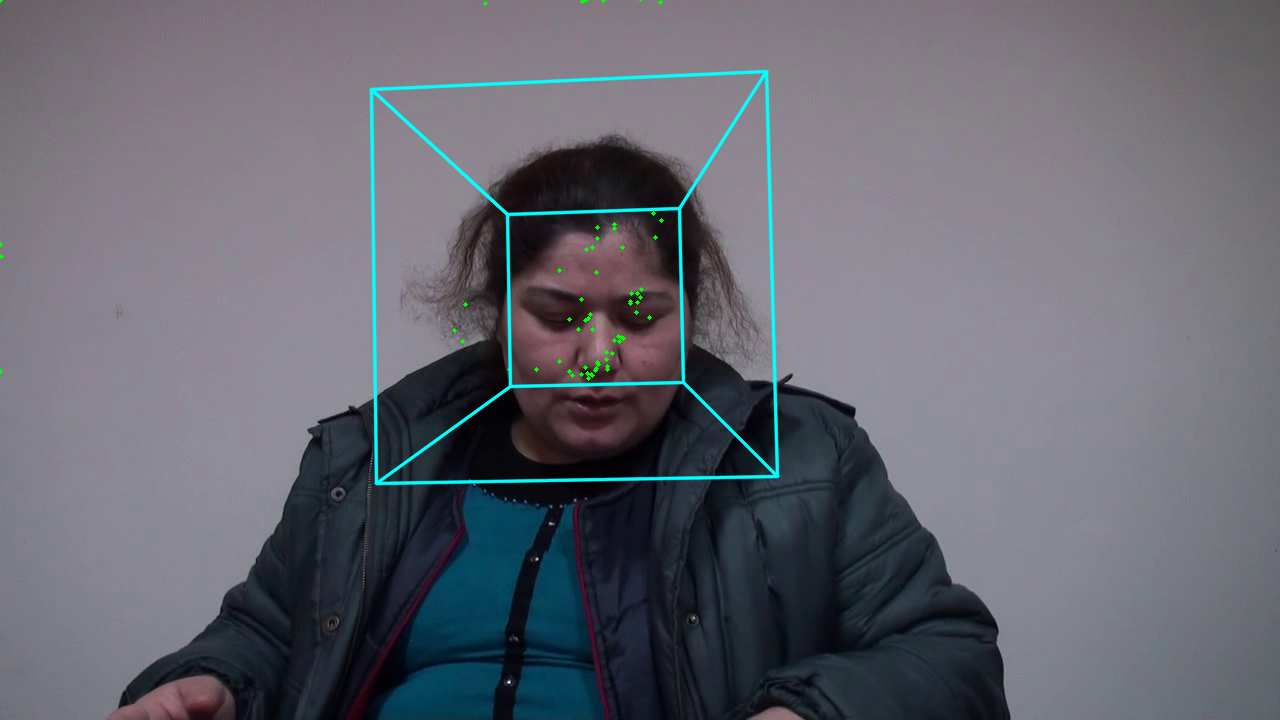
\includegraphics[width=\textwidth]{images/facial/recons_285_face_0_multiDDAE_mfcc.png} \\
    (d) reconstructed input at frame 285 from (1) in Table \ref{tab:multimodal_res}
    \end{minipage}
    \\
    \begin{minipage}[c]{0.42\linewidth}
    \centering
    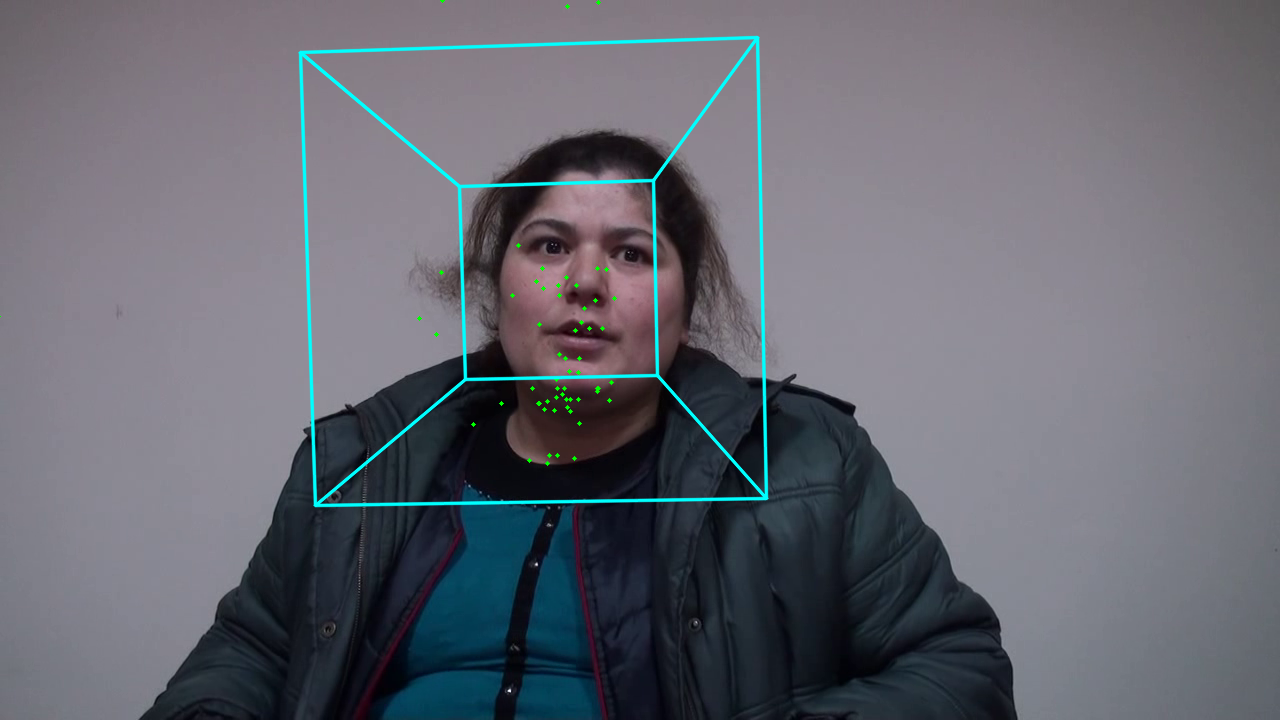
\includegraphics[width=\textwidth]{images/facial/recons_45_face_0_multiDDAE_egemaps.png} \\
    (e) reconstructed input at frame 45 from (10) in Table \ref{tab:multimodal_res}
    \end{minipage}
    \begin{minipage}[c]{0.42\linewidth}
    \centering
    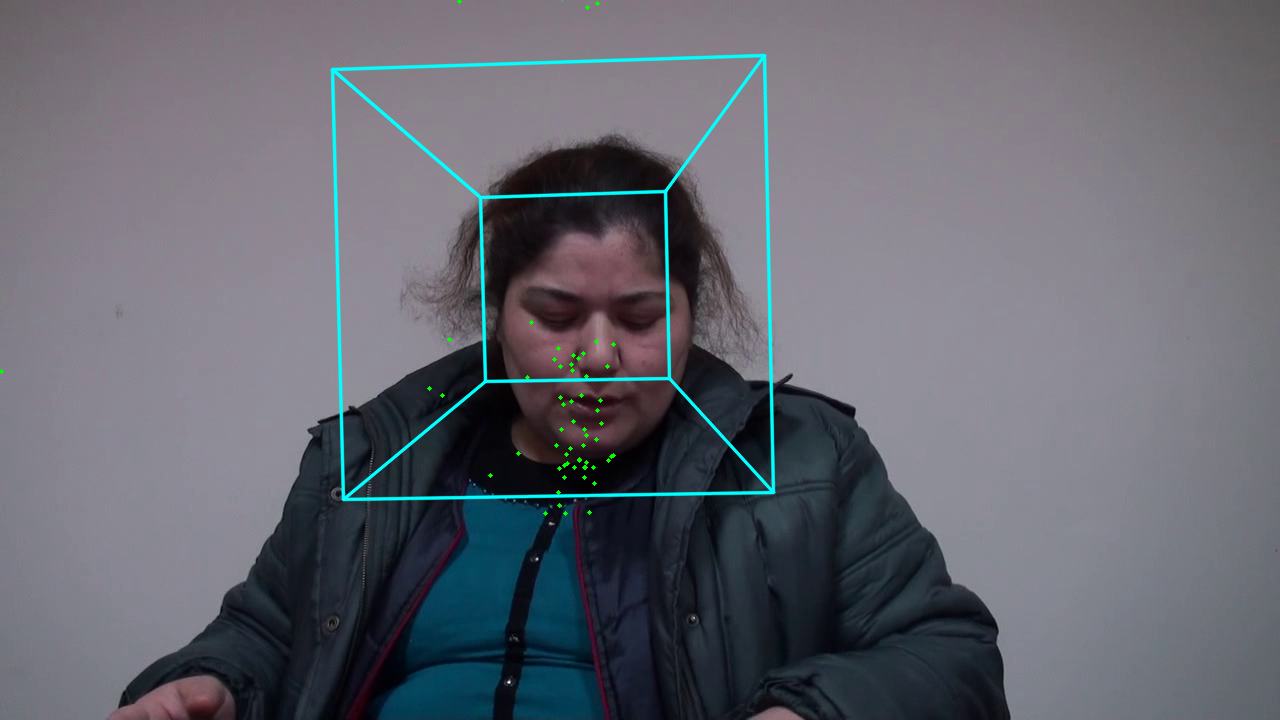
\includegraphics[width=\textwidth]{images/facial/recons_285_face_0_multiDDAE_egemaps.png} \\
    (f) reconstructed input at frame 285 from (10) in Table \ref{tab:multimodal_res}
    \end{minipage}
    \caption{Reconstruction of facial landmarks and head pose in Multimodal DDAEs from noisy input}
    \label{fig:reconstruction_multiDDAE}
\end{figure}


T-distributed Stochastic Neighbour Embedding (t-SNE) was proposed for dimensionality reduction and visualization of high-dimensional data in two or three dimensions \cite{maaten2008}. These following visualizations are generated using the Embedding Projector (\url{https://projector.tensorflow.org/}) with approximately 1000 iterations and 0.01 learning rate.

Before measuring the classification performance, Fisher Vectors (FVs) after feature selection are visualized via t-SNE as Figure \ref{fig:tsne_DDAEs}, which only concentrates on the best-performing bi-DDAEs and multi-DDAEs in Table \ref{tab:bimodal_res} and \ref{tab:multimodal_res}. As shown in Figure \ref{fig:tsne_DDAEs}, three, four, and five clusters can be easily identified in (a), (c) and (d) respectively that validate the better performance of DDAE architectures except bi-DDAE on eGeMAPS, whose visualization fails to show clear clusters in (b). In addition, DDAEs using MFCC as acoustic features help to produce more discriminative FVs (seen in (a) and (c)), which corresponds to the better performance on (1) in both \ref{tab:bimodal_res} and \ref{tab:multimodal_res}. The best performance of (1) in Table \ref{tab:multimodal_res} is validated through the visualization of FVs.


\begin{figure}[htb]
    \centering
    \small
    \begin{minipage}[c]{0.4\linewidth}
    \centering
    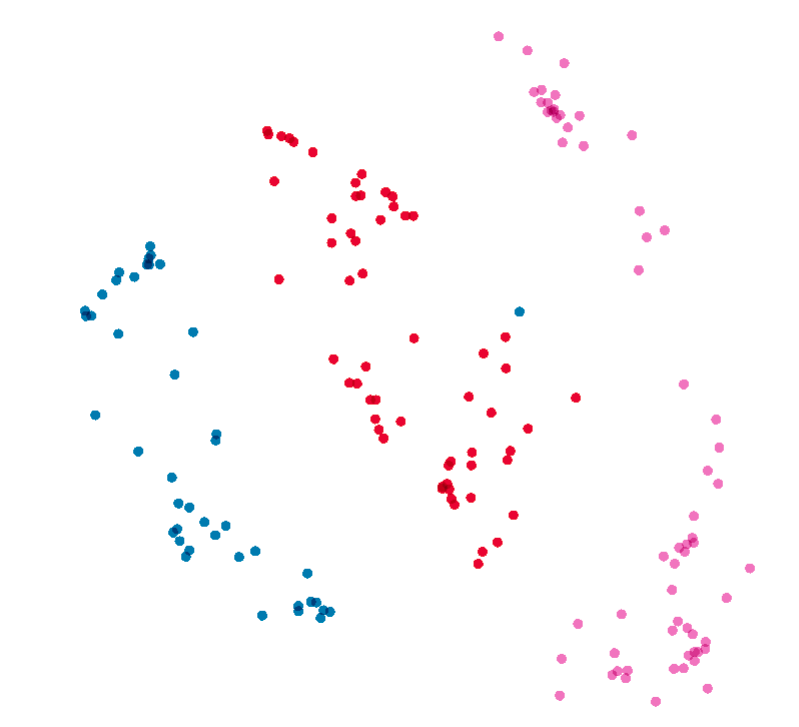
\includegraphics[height=4.8cm]{images/results/bi_DDAE_MFCC_tsne.png} \\
    (a) bi-DDAE (1) in Table \ref{tab:bimodal_res}
    \end{minipage}
    \begin{minipage}[c]{0.4\linewidth}
    \centering
    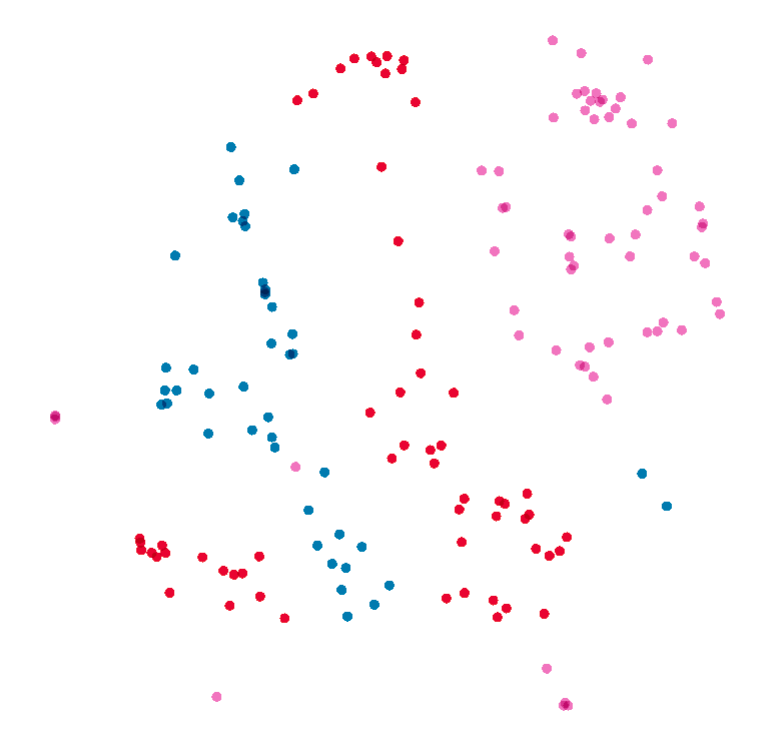
\includegraphics[height=4.8cm]{images/results/bi_DDAE_eGeMAPS_tsne.png} \\
    (b) bi-DDAE (10) in Table \ref{tab:bimodal_res}
    \end{minipage}
    \\
    \begin{minipage}[c]{0.4\linewidth}
    \centering
    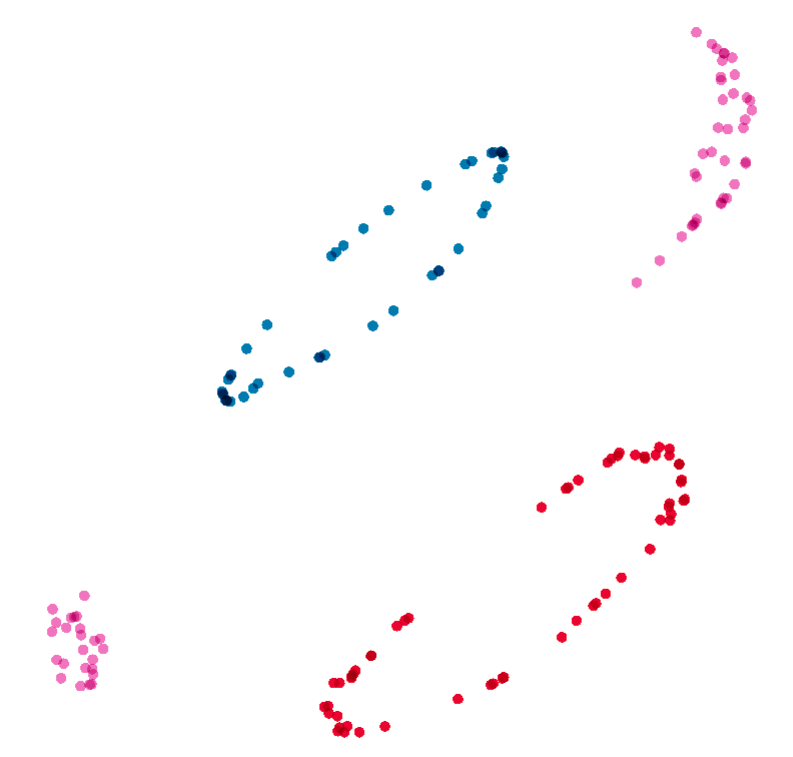
\includegraphics[height=4.8cm]{images/results/multi_DDAE_MFCC_tsne.png} \\
    (c) multi-DDAE (1) in Table \ref{tab:multimodal_res}
    \end{minipage}
    \begin{minipage}[c]{0.4\linewidth}
    \centering
    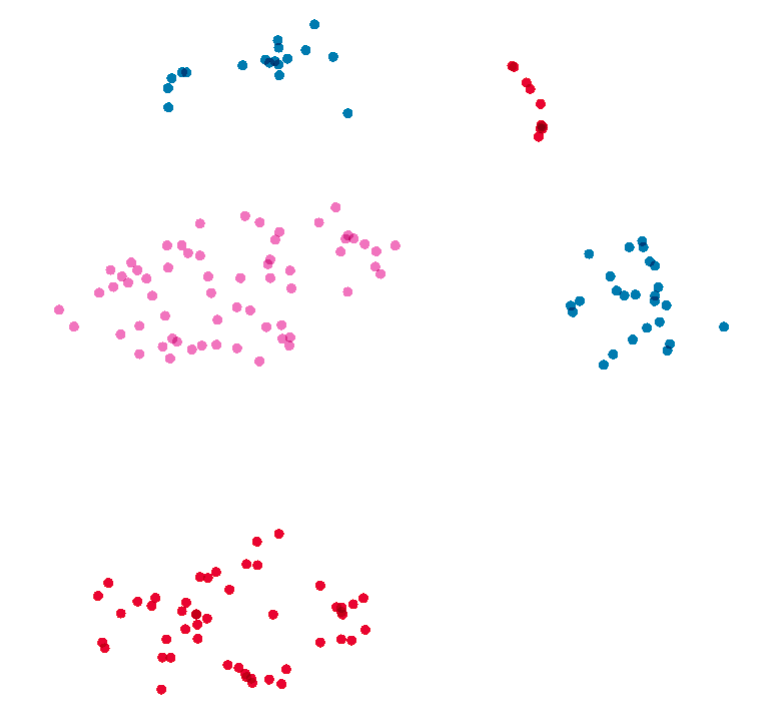
\includegraphics[height=5.1cm]{images/results/multi_DDAE_eGeMAPS_tsne.png} \\
    (d) multi-DDAE (10) in Table \ref{tab:multimodal_res}
    \end{minipage}
    \caption{Fisher vectors visualization in 2D space using t-SNE algorithm}
    \label{fig:tsne_DDAEs}
\end{figure}



\section{Textual Modality}

In the textual modality, the classification performance of different hyperparameter settings of document embeddings is represented first and the same Random Forest (RF) as the baseline are used for the classification. To evaluate the quality of document embeddings, I visualize the embedding space and list the word similarities and the document similarities, which are inferred by the embedding models. 

\subsection{Assessment of document embeddings}

Table \ref{tab:doc2vec_res} presents the experimental results for the document embedding models on the transcripts of interview sessions, and only the best-performing hyperparameter setting in both doc2vec models is listed. The full comparison of doc2vec models with different hyperparameter settings refers to Table \ref{tab:doc2vec_results} in Appendix and it is also visualized in a barchart as Figure \ref{fig:doc2vec_bar}.  


\begin{figure}[ht]
    \centering
    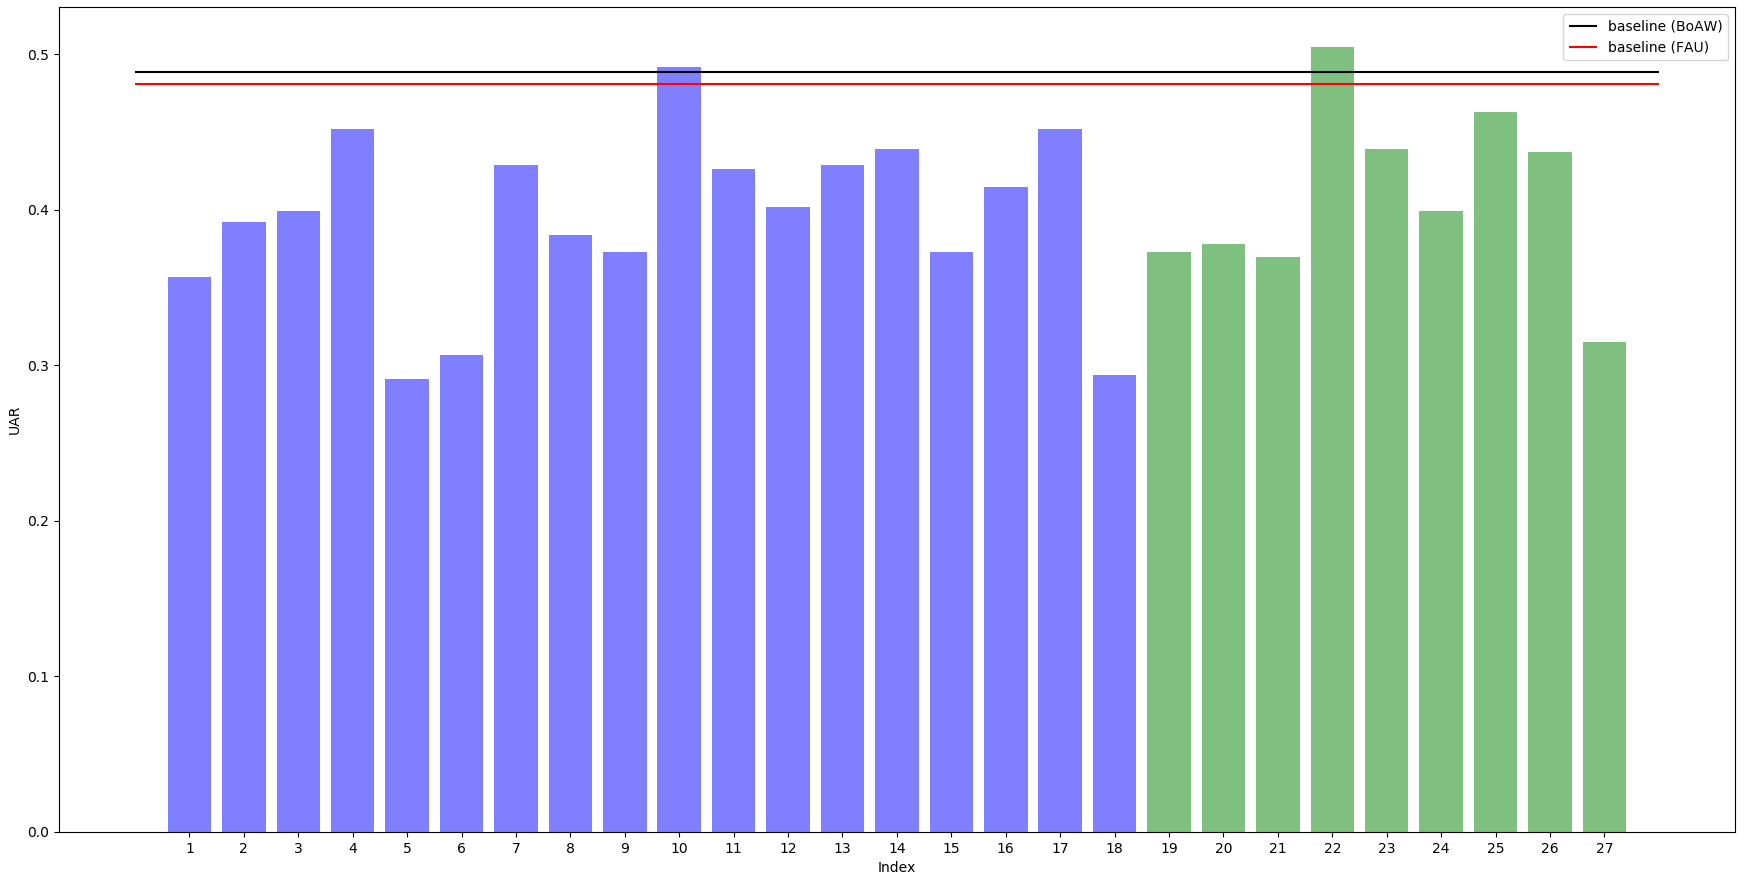
\includegraphics[width=\textwidth]{images/results/doc2vec.png}
    \caption{Barchart for the experimental results of doc2vec models indexed as Table \ref{tab:doc2vec_results}}
    \label{fig:doc2vec_bar}
\end{figure}

As illustrated in Table \ref{tab:doc2vec_res}, both PV-DM and PV-DBOW models achieve slightly better performance than the baseline. As their performance on sentiment analysis task \cite{lau2016}, the experimental results in BD recognition task show better performance in PV-DBOW in comparison with PV-DM (0.013 higher in UAR and 0.038 in F1 score). 
Additionally, I find that PV-DBOW models generally outperform PV-DM models in the hyperparameter settings as shown in Figure \ref{fig:doc2vec} and only the selected PV-DBOW and PV-DM models outperform the baseline while others do not.


\begin{table}[htb]
    \centering
    \small
    \caption{Comparison of proposed document embeddings on the transcripts (selected experimental results) with baseline results attached}
    \begin{tabular}{l|l|p{1.2cm}|p{1.5cm}|p{1.6cm}|l|l|l}
    \Xhline{2\arrayrulewidth}
        Index & Model & Vector size & Window size & Negative words & UAR & UAP & F1 \\
        \hline
        (10) & PV-DM & 50 & 10 & 5 & 0.492 & 0.481 & 0.486 \\
        \hline
        (22) & PV-DBOW & 50 & - & 5 & 0.505 & 0.544 & 0.524 \\
        \hline
        & \multicolumn{4}{l|}{Baseline (BoAW)} & 0.489 & 0.439 & 0.463 \\
        & \multicolumn{4}{l|}{Baseline (FAU)} & 0.481 & 0.528 & 0.503 \\
    \Xhline{2\arrayrulewidth}
    \end{tabular}
    \label{tab:doc2vec_res}
\end{table}



\subsection{Visualization and Qualitative Analysis}

The cosine similarity between similar words is first examined as Table \ref{tab:word_similarity}, in which top five similar words inferred by doc2vec models ((10) and (22) in Table \ref{tab:doc2vec_res}) with the target word 'good' are listed along with the translation. The similarity $|x - y|$ and distance $\langle x,y \rangle$ between two words are defined as $|x-y|^2 = |x|^2 + |y|^2 - 2\langle x,y\rangle$. Therefore, in the embedding space of doc2vec models, similar words should have high cosine similarity and a short distance between each other. 

As seen in Table \ref{tab:word_similarity}, the PV-DM model indeed shows a more meaningful embedding results as 'high', 'good' and 'important' are generally considered to be positively related with 'good' while 'least' and 'little' are considered to be negatively related. This indicates that words with similar meanings are mapped to similar positions in the embedding space \cite{mikolov2014}. On the other hand, the similar words inferred by PV-DBOW are not related to the word 'good' as the PV-DBOW model does not train the word vectors and these vectors remain randomly initialized values.


\begin{table}[htb]
    \centering
    \small
    \caption{Word similarities inferred by doc2vec models}
    \begin{tabular}{l|p{1cm}|p{1.5cm}|p{1.5cm}|p{1.5cm}|p{1.7cm}|p{1.5cm}}
        \Xhline{2\arrayrulewidth}
        \multicolumn{7}{l}{PV-DM} \\
        \Xhline{2\arrayrulewidth}
        word & \textbf{iyi} & azından & yüksek & iyisi & az & önemlisi \\
        \hline
        translation & \textbf{good} & least & high & good & little & important \\
        \hline
        similarity & - & 0.894 & 0.869 & 0.862 & 0.853 & 0.825 \\
        \Xhline{2\arrayrulewidth}
        \multicolumn{7}{l}{PV-DBOW} \\
        \Xhline{2\arrayrulewidth}
        word & \textbf{iyi} & yul bugavi & düşünü- lebir & ikamet- gahlarına & hastalıktır & içereni \\
        \hline
        translation & \textbf{good} & followings & it is considered of & to residence & disease & including \\
        \hline
        similarity & - & 0.613 & 0.607 & 0.603 & 0.599 & 0.589 \\
        \Xhline{2\arrayrulewidth}
    \end{tabular}
    \label{tab:word_similarity}
\end{table}


To extend the similarity from word-level to document-level, I randomly select one transcript of the interview session and use doc2vec models to inferred the similar documents, which should be also mapped to similar position in the embedding space \cite{mikolov2014}. Table \ref{tab:doc_sim_dm} presents the most similar and the least similar transcripts inferred by PV-DM to the target and Table \ref{tab:doc_sim_dbow} presents the same information but inferred by PV-DBOW. These two tables are attached at the end of this chapter. Since the mental state information exists in textual modality, the most similar transcript and the target in Table \ref{tab:doc_sim_dm} show a similar sentiment or emotion of the interviewee that he/she could be upset, helpless, or worried. The least similar transcript, however, shows nothing related to the target. Based on the same target, Table \ref{tab:doc_sim_dbow} shows that PV-DBOW maps transcripts to an embedding space in which similar transcripts share similar feelings of the subject.


\begin{figure}[htb]
    \centering
    \small
    \begin{minipage}{0.42\linewidth}
    \centering
    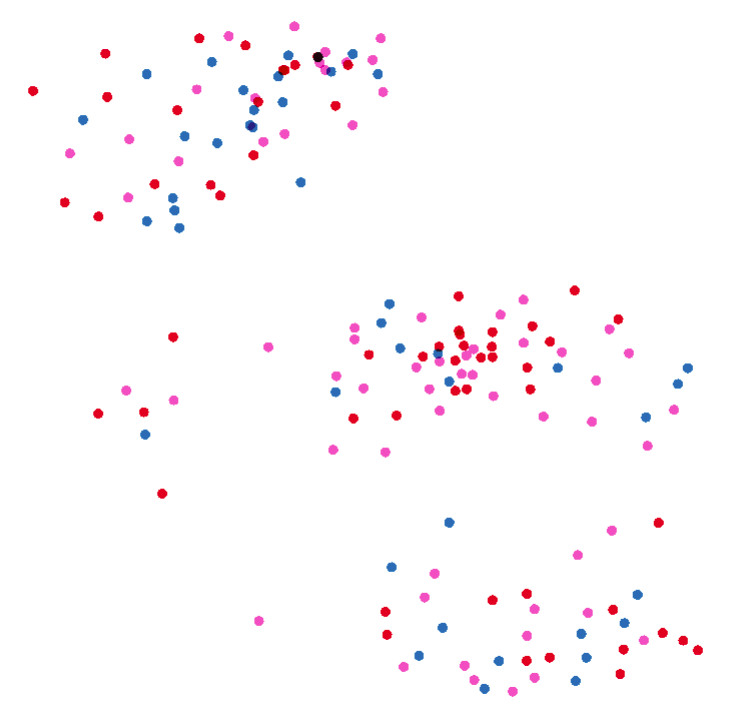
\includegraphics[width=6cm]{images/results/dm_tsne_2d.png} \\
    (a) PV-DM ((10) in Table \ref{tab:doc2vec_res})
    \end{minipage}
    \hfill
    \begin{minipage}{0.42\linewidth}
    \centering
    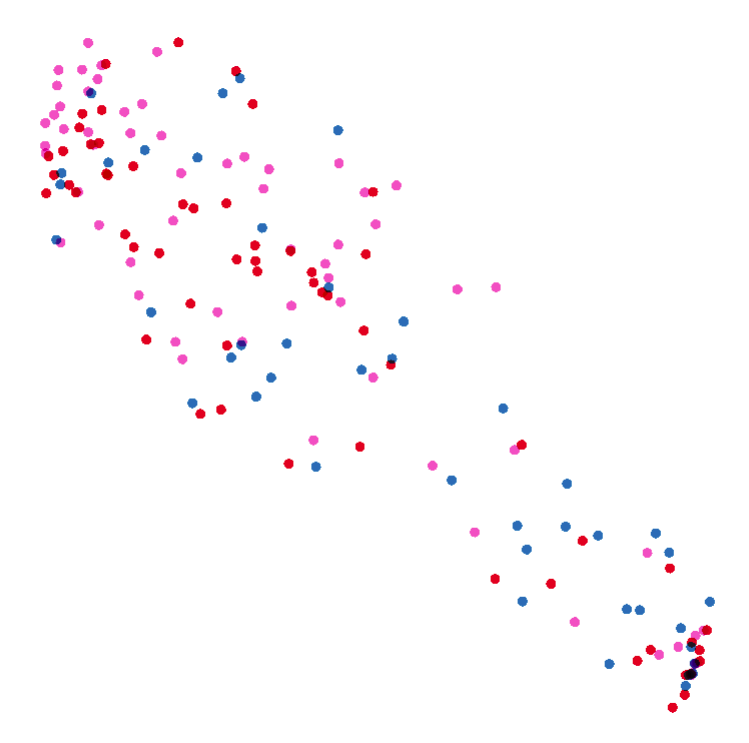
\includegraphics[width=6cm]{images/results/dbow_tsne_2d.png} \\
    (b) PV-DBOW ((22) in Table \ref{tab:doc2vec_res})
    \end{minipage}
    \caption{Document embeddings visualization in 2D space using t-SNE algorithm}
    \label{fig:doc2vec_vis_tsne}
\end{figure}


Similar as the visualization of Fisher Vectors (FVs), Figure \ref{fig:doc2vec_vis_tsne} displays the t-SNE visualization in 2-dimensional space for doc2vec models. The visualization is completed using the Embedding Projector (\url{https://projector.tensorflow.org/}) with around 1000 iteration and 0.01 learning rate. The colours in Figure \ref{fig:doc2vec_vis_tsne} indicate the same classes, of which the data points should be close to one another. Four clusters can be observed in (a) of Figure \ref{fig:doc2vec_vis_tsne} and two clusters in (b). There are, however, data points of more than one class in each cluster that impair the separation between different classes. This could account for the performance of doc2vec models on the classification of BD symptoms.


\section{Multimodal Feature Fusion}

With bi-DDAEs and multi-DDAEs on audio-visual modality and doc2vec models on textual modality, a total of 8 combinations are presented as Table \ref{tab:fusion_res}, in which the bi-DDAEs, multi-DDAEs and doc2vec models are the best-performing ones corresponding to Table \ref{tab:bimodal_res}, Table \ref{tab:multimodal_res} and Table \ref{tab:doc2vec_res} respectively.

\begin{table}[htb]
    \centering
    \small
    \caption{Comparison of proposed framework with feature fusion on audio-visual modality and textual modality. The best performance is in \textbf{bold} for each metric.}
    \begin{tabular}{l|l|l|l|l|l}
    \Xhline{2\arrayrulewidth}
        Index & Audio-Visual modality & Textual modality & UAR & UAP & F1  \\
        \hline
        (1) & bi-DDAE (MFCC) & PV-DM & 0.659 & 0.683 & 0.671 \\
        (2) & bi-DDAE (MFCC) & PV-DBOW & 0.593 & 0.602 & 0.597 \\
        (3) & bi-DDAE (eGeMAPS) & PV-DM & 0.571 & 0.624 & 0.596 \\
        (4) & bi-DDAE (eGeMAPS) & PV-DBOW & 0.603 & 0.633 & 0.618 \\
        (5) & multi-DDAE (MFCC) & PV-DM & \textbf{0.709} & \textbf{0.734} & \textbf{0.721} \\
        (6) & multi-DDAE (MFCC) & PV-DBOW & 0.667 & 0.680 & 0.673 \\
        (7) & multi-DDAE (eGeMAPS) & PV-DM & 0.675 & 0.708 & 0.691 \\
        (8) & multi-DDAE (eGeMAPS) & PV-DBOW & 0.659 & 0.671 & 0.665 \\
    \Xhline{2\arrayrulewidth}
    \end{tabular}
    \label{tab:fusion_res}
\end{table}

The early fusion strategy is applied to concatenate the compact-size vectors from audio-visual modality and textual modality to obtain a joint feature for the Multi-Task Neural Network (MTNN). The dimension of fused features is 150, the sum of 100-dimensional audio-visual features after feature selection and 50-dimensional document embeddings. The MTNN is then fine-tuned on the pre-determined development set with overfitting addressed. As Table \ref{tab:fusion_res} shows, the best performing framework is based on the fusion of (1) multi-DDAE using MFCC as acoustic features and (10) PV-DM document embeddings and the UAR reaches up to 0.709 and F1 score to 0.721. 

While PV-DBOW alone performs better than PV-DM, PV-DM fused with DDAEs shows a higher UAR and F1 score than PV-DBOW fused with DDAEs, indicating complementary mental information appended to the fused feature.



\subsection{Comparison with Competing Frameworks}

Since the experiments are based on the pre-determined partition of the BD corpus, the proposed framework can be directly compared with the frameworks proposed in AVEC2018 \cite{ringeval2018}. Table \ref{tab:avec2018_compare} lists the experimental results produced by different frameworks on the development set. It is clear that my framework outperforms the frameworks proposed by \cite{du2018} and \cite{syed2018} in both UAR and accuracy. Furthermore, my framework achieves the same accuracy as \cite{yang2018} with a very close UAR (only 0.005 lower). Therefore, the proposed framework, which is based on a multi-DDAE to encode audio-visual modality and a PV-DM to embed textual modality, achieves the state-of-the-art performance on BD recognition.

\begin{table}[h]
    \small
    \centering
    \caption{Comparison of the proposed framework (which performance is in \textbf{bold}) with the competing frameworks in AVEC2018}
    \begin{tabular}{l|l|l}
    \Xhline{2\arrayrulewidth}
        Framework & UAR (dev) & Accuracy (dev) \\
        \hline
        Yang \textit{et al.} 2018 & 0.714 & 0.717 \\
        \hline
        Du \textit{et al.} 2018 & 0.651 & 0.650 \\
        \hline
        Xing \textit{et al.} 2018 & 0.868 & NA \\
        \hline
        Syed \textit{et al.} 2018 & 0.635 & NA \\
        \hline
        \textbf{This work} 2019 & \textbf{0.709} & \textbf{0.717} \\
    \Xhline{2\arrayrulewidth}
    \end{tabular}
    \label{tab:avec2018_compare}
\end{table}


\subsection{Generalization}

To validate the generalization of the proposed framework, a 10-fold cross-validation is implemented for 8 frameworks listed in Table \ref{tab:fusion_res}. As there are $104 + 60 = 164$ samples in the corpus, 16 samples are selected as the test set with the rest as the training set. In Figure \ref{fig:errorbar}, the index of frameworks corresponds to Table \ref{tab:fusion_res}, in which (5) performs the best on pre-determined development set. 

Figure \ref{fig:errorbar} displays the means, visualized as bars, and the variances, visualized as error bars, which are calculated from the UAR on 10-fold cross-validation of different fusion frameworks. It is worth noting that (5) fusion framework still has the highest averaged UAR at approximately 0.60 and it can reach up to 0.91 UAR in one train/test split. For the rest of fusion frameworks, the averaged UAR in (3) and (4) is slightly higher than 0.50 and the second best-performing one, (7) has only the average UAR over 0.54. Therefore, framework (3), (4) and (7) are demonstrated less effective than others, and more likely to suffer from overfitting to the train/test split defined in AVEC2018. 

\begin{figure}[htb]
    \centering
    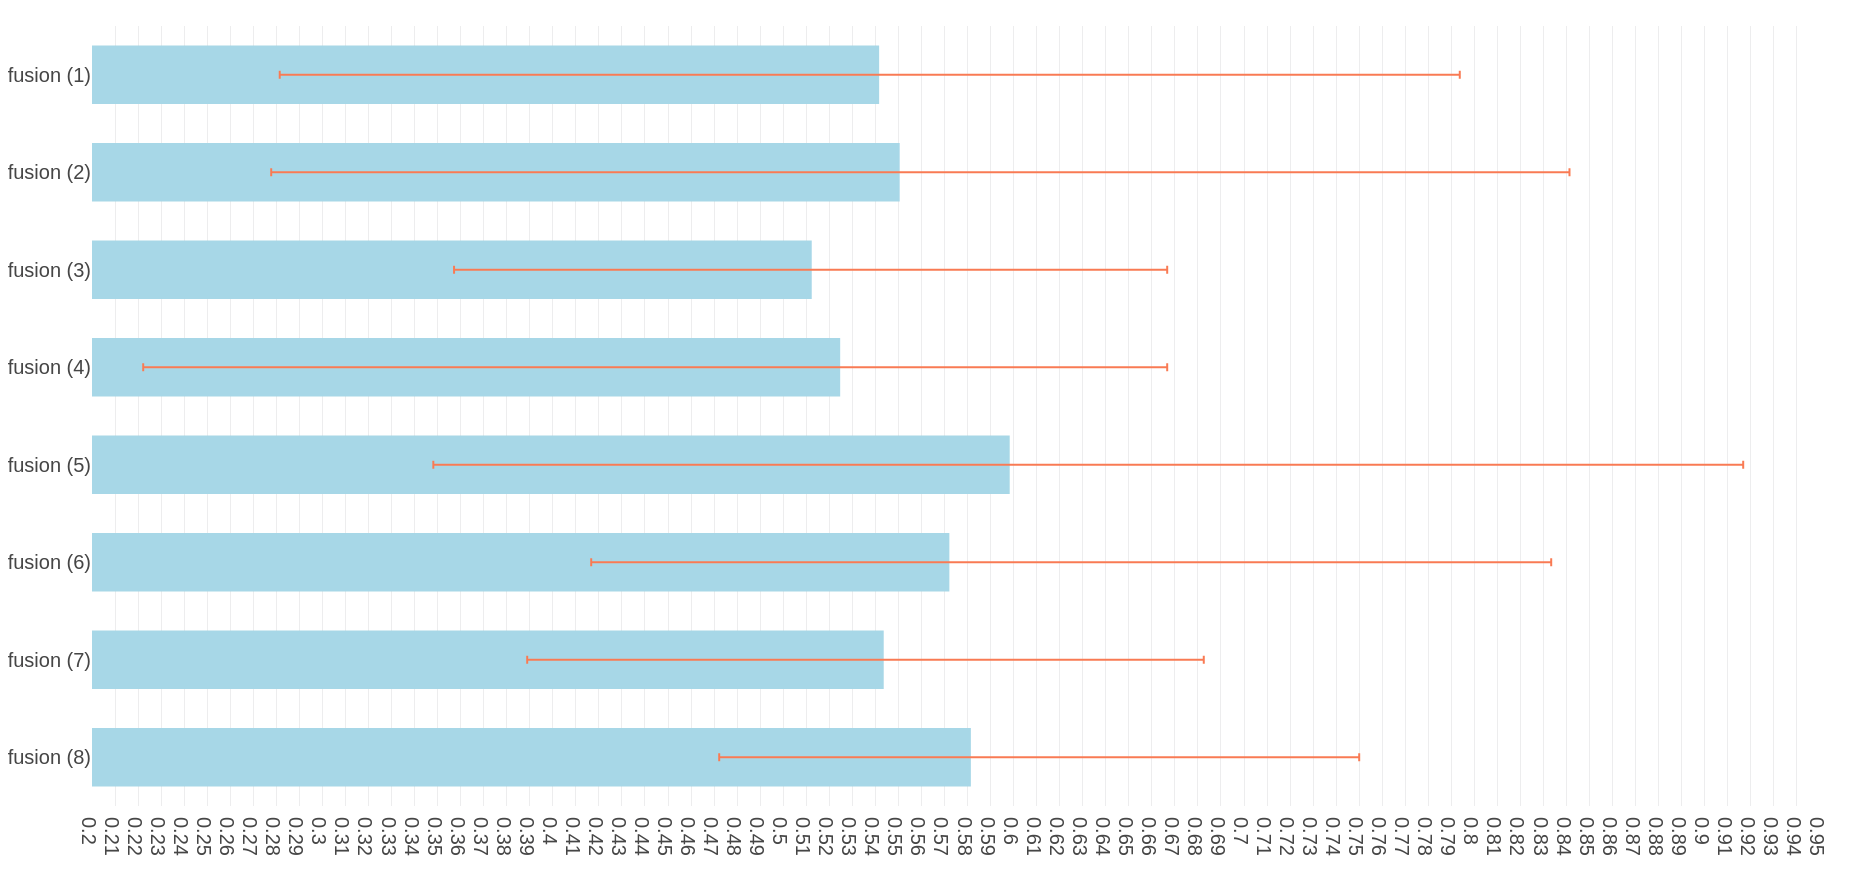
\includegraphics[width=\textwidth]{images/results/barchart_cv.png}
    \caption{Barchart of the averaged UAR and variance generated via a 10-fold cross-validation on different fusion frameworks}
    \label{fig:errorbar}
\end{figure}




\begin{table}[h]
    \centering
    \small
    \caption{Document similarities inferred by PV-DM model}
    \begin{tabular}{p{6.5cm}|p{6cm}}
        \Xhline{2\arrayrulewidth}
        \textless Target\textgreater ...görüştükten sonra bu tarafa geçirdiler Ben dediğimi burada ızdırap çeken bir insan var ya yanında bir portre var bunun kalemler falan var öyle Alev yanarken alevler çıkarkenki bir yanıt var bilmiyorum ama neden çok çaresiz çok çaresiz duruyor yani sanki yüzünü insanın yüzüne bakmaya yüzü kalmamış gibi kafasını falan aynı rahmetli babama da benzettim yanında çaresiz bir insan görüyorum burada çok çaresiz ne yapacağını bilmeyen kendine şaşırmış bir tek sandalyesi... & \textless Translation\textgreater ...There is a person who suffers from what I said here or there is a portrait of it. There is a pencil or something. I don't know why there is an answer while the flame is burning, but why is it so desperate and so desperate, it's as if you don't have a face to face. I've seen a helpless person next to my deceased father likened here too helpless does not know what to do self-surprised single chair... \\
        \hline
        \multicolumn{2}{l}{Similarity: 0.796} \\
        \hline
        \textless Most Similar\textgreater ...Bir hatırlatır misiniz Annemi babamı üzmem en büyük yanlış ve toplumla yargıda aradı davrandı için toplumu kafaya taktım saplantı yaptım mutlu ve aile tablosu bu sorunu daha önce de soruldu arkadaşa bir doğum günü şakası yapmıştı koydum en güzel hatıra... & \textless Translation\textgreater ...Could you remind me of my mother to upset my father the biggest wrong and looked for the society in the judiciary pretended I was obsessed with the society and the family table was happy before I was asked this problem a friend had made a birthday joke I said the most beautiful souvenir... \\
        \hline
        \multicolumn{2}{l}{Similarity: -0.031} \\
        \hline
        \textless Least Similar\textgreater ...Hepsi- burada evlendiniz mi Anlatır mısınız ya ne düşündüğünü ve istediğini üzere bir adamla ağlıyor gibi kötü teşekkür ederiz... & \textless Translation\textgreater ...Did you ever marry here? Can you tell me or thank you badly as if you are crying with a man as he thinks and wants?... \\
        \Xhline{2\arrayrulewidth}
    \end{tabular}
    \label{tab:doc_sim_dm}
\end{table}

\begin{table}[h]
    \centering
    \small
    \caption{Document similarities inferred by PV-DBOW model}
    \begin{tabular}{p{6.5cm}|p{6cm}}
        \Xhline{2\arrayrulewidth}
        \textless Target\textgreater ...görüştükten sonra bu tarafa geçirdiler Ben dediğimi burada ızdırap çeken bir insan var ya yanında bir portre var bunun kalemler falan var öyle Alev yanarken alevler çıkarkenki bir yanıt var bilmiyorum ama neden çok çaresiz çok çaresiz duruyor yani sanki yüzünü insanın yüzüne bakmaya yüzü kalmamış gibi kafasını falan aynı rahmetli babama da benzettim yanında çaresiz bir insan görüyorum burada çok çaresiz ne yapacağını bilmeyen kendine şaşırmış bir tek sandalyesi... & \textless Translation\textgreater ...There is a person who suffers from what I said here or there is a portrait of it. There is a pencil or something. I don't know why there is an answer while the flame is burning, but why is it so desperate and so desperate, it's as if you don't have a face to face. I've seen a helpless person next to my deceased father likened here too helpless does not know what to do self-surprised single chair... \\
        \hline
        \multicolumn{2}{l}{Similarity: 0.879} \\
        \hline
        \textless Most Similar\textgreater ...Pardon unuttum tablosu değil Mutsuz bir aile tablosu oda dolusu veri tablosu çocuklarıyla ve eşiyle mutlu arada güçlü bir sevgi bağı var doğru mu Buse Bu kadar yeter yaşamımızdaki en güzel hatırınız anlatır mısın vallahi öyle yaşamındaki en güzel hatıram alkollüydü arkadaşlarla kafamız sarhoşluk yani kafam iyi değil Çok sarhoştum güzel bir arkadaşlık arkaya vurulmuştu ama o espriyi Söyleyemem çok oturdum güzel bir espri yapmıştım da arkadaşlarımı Espriye görmüştü... & \textless Translation\textgreater ...Sorry I forgot the table is not an unhappy family table room full of data table Is there a strong bond of love between the children and his wife happy Buse Do you tell me the most beautiful memory in our life, I swear that the most beautiful memories of life in my life was drunk with friends I was very drunk a beautiful friendship was shot in the back, but I can not say that joke sat a nice joke I had seen my friends joke... \\
        \hline
        \multicolumn{2}{l}{Similarity: 0.171} \\
        \hline
        \textless Least Similar\textgreater ...Hepsi- burada evlendiniz mi Anlatır mısınız ya ne düşündüğünü ve istediğini üzere bir adamla ağlıyor gibi kötü teşekkür ederiz... & \textless Translation\textgreater ...Did you ever marry here? Can you tell me or thank you badly as if you are crying with a man as he thinks and wants?... \\
        \Xhline{2\arrayrulewidth}
    \end{tabular}
    \label{tab:doc_sim_dbow}
\end{table}
